\chapter{Design}

\section{Overall System Design}

\subsection{Short description of the main parts of the system}

Hardware Allocation Database

\begin{itemize}
\item IT staff user interface
\item Line manager user inferface
\item Staff user interface
\item Login screen
\item Viewing Databases
\item Editing Databases \& Adding and Deleting data
\end{itemize}

\

\textbf{IT staff user interface}

\begin{itemize}
\item IT staff have admin rights to the system. They will be able to view everyones information and are the only people who may edit information on the system.
\item Once logged in they will be presented with a user interface with buttons allowing them to open a database or search for staff.
\item All IT staff will share a username and password.
\item The search function will take the user to an interface which will allow them to search for a staff member and be shown which hardware devices they own. This search could also be performed by going to the staff database and using the search function there, but this may be used frequently and so is placed here for convience.
\item The open database button will take them to a user interface that will have a dropdown box allowing them to pick which database to view. There will be Edit, Add and Remove options available when a database is shown. A search button will also be on this screen to allow the user to search for a specific field.
\item The edit database will allow the user to change information on the database.
\item The add data will allow the user to add new records
\item The remove data will allow the user to delete records
\end{itemize}

\

\textbf{Line manager user interface}

\begin{itemize}
\item Line manager's have more rights than normal staff but unlike IT staff they cannot edit any information.
\item Line manager's share the same username if they are part of the same department and the same location (liverpool and orwell cannot use the same department login) and a password that they may change at any time. Upon first using the system their password will be issued by IT staff. Their username at the moment will be a 5 digit number allocated to them by IT staff, however this username may change depending on the users needs. (the best way to do this will be via email). 
\item Line manager's can view information of members from their own department.
\item Once logged in, the user interface will show a "View Department" button and a "View My Information" button.
\item The "View Department" button will show the staff database but only show records from staff at their own department. There will be a search function to find a specific field.
\item The "View My Information" button will allow the user to view their own hardware devices and personal information. It may be used often to check the warranty period of an item and to check correct information is being displayed.
\end{itemize}

\

\textbf{Staff User Interface}
\begin{itemize}
\item Ordinary staff members will all have unique usernames and be able to create their own password.
\item After logging on they will be taken immediatly to the table showing their own information. The system does not allow staff to do much so it is best to keep things very simple.
\item  They may use the search bar to query information
\end{itemize}

\

\textbf{Login screen}
\begin{itemize}
\item The login screen will have a username field and a password field. There will also be two buttons, one to login and the other will be "Forgot Your Password?".
\item The "Forgot Your Password?" button will take the user to another interface which will ask for their Volac (company) email address, Forename and Surname. This information will be sent to the IT staff who can review it and email the user another password to use or tell them what their password was. It is important to note that all Volac staff have the same buisness email (for example XXX.Volac.com), this means SMTP settings can be set up easily in Python. This process will be easier than asking IT Staff directly.
\item Normal staff all have their own username and a password that they may change at any time. Upon first using the system their password will be issued by IT staff. Their username will be a 5 digit number allocated to them by IT staff (the best way to do this will be via email). 
\item Line manager's share the same username if they are part of the same department and location, the password they may change at any time. Upon first using the system their password will be issued by IT staff. Their username will be a 5 digit number allocated to them by IT staff (the best way to do this will be via email). 
\item All IT staff will share a username and password to have admin rights.
\item There are 100,000 combinations on a 5 digit number (10$^5$) which will be more than enough for the company (if I was to use this mehtod), it will be best to start from the left and issue 10000 to IT staff and start with 20000 for other staff (and proceed with 20001, 20002, ... 20010...)
\end{itemize}

\

\textbf{Viewing Databases}

\begin{itemize}
\item All staff, in some way, will be able to view a database.
\item For general staff, they will only be able to view their own data. Line Manager's will be able to view all data in the staff database about the members in their department. IT staff have full access to all databases to view all information.
\item A dropdown box will be useful for IT staff to pick a database to view, buttons will surffice for other staff since they can only view a couple of databases.
\end{itemize}

\

\textbf{Editing Databases}
\begin{itemize}
\item To edit existing entries the user will click the "Edit Database" button (found on the IT staff/admin interface).
\item To add new data they will click "Add Data"take the user to a form which allows data to be input into fields for such things as First Name, Surname, Warranty or Hardware Device.
\item To remove data they will click "Remove Data" and then can choose the record to remove.
\item Validation will be required for various fields such as telephone numbers (string of length 11) and dropdown boxes will be used for boolean values for fields such as Warranty.
\end{itemize}


\subsection{System flowcharts showing an overview of the complete system}

\begin{figure}[H]
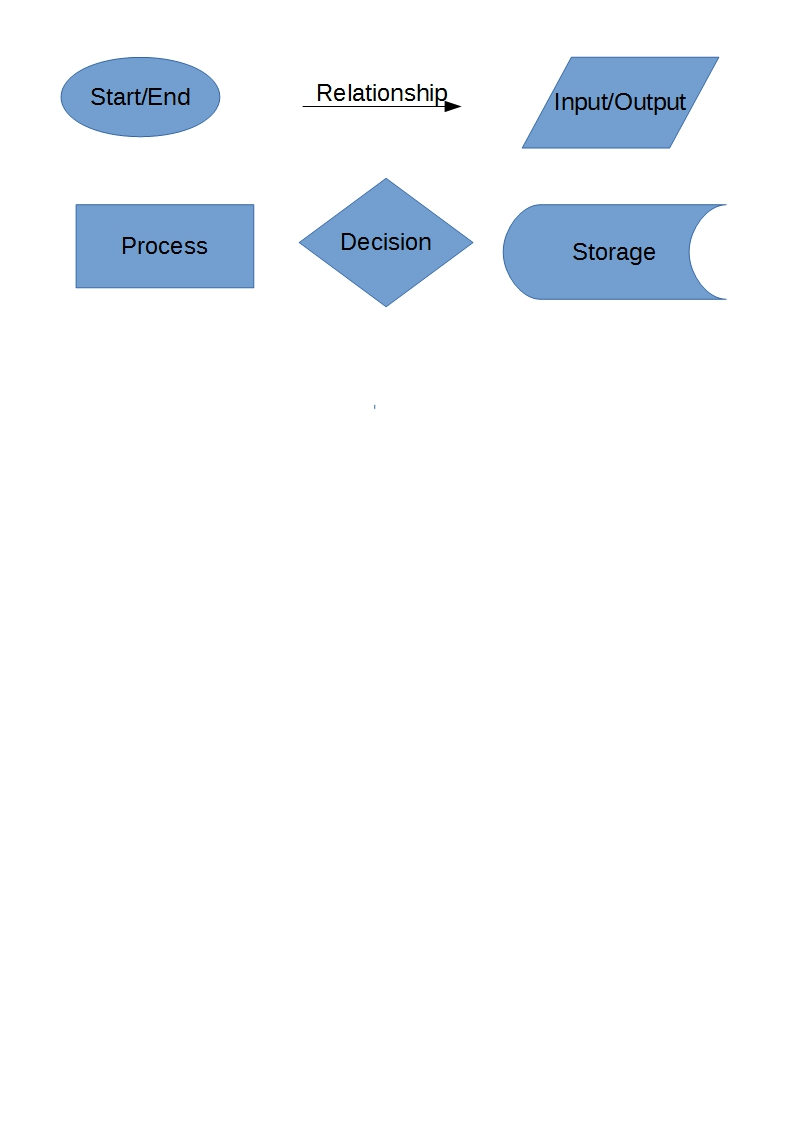
\includegraphics[width=.9\textwidth,height=.9\textheight,keepaspectratio]{FlowchartKey.jpg}
\end{figure}

\newpage

\begin{figure}[H]
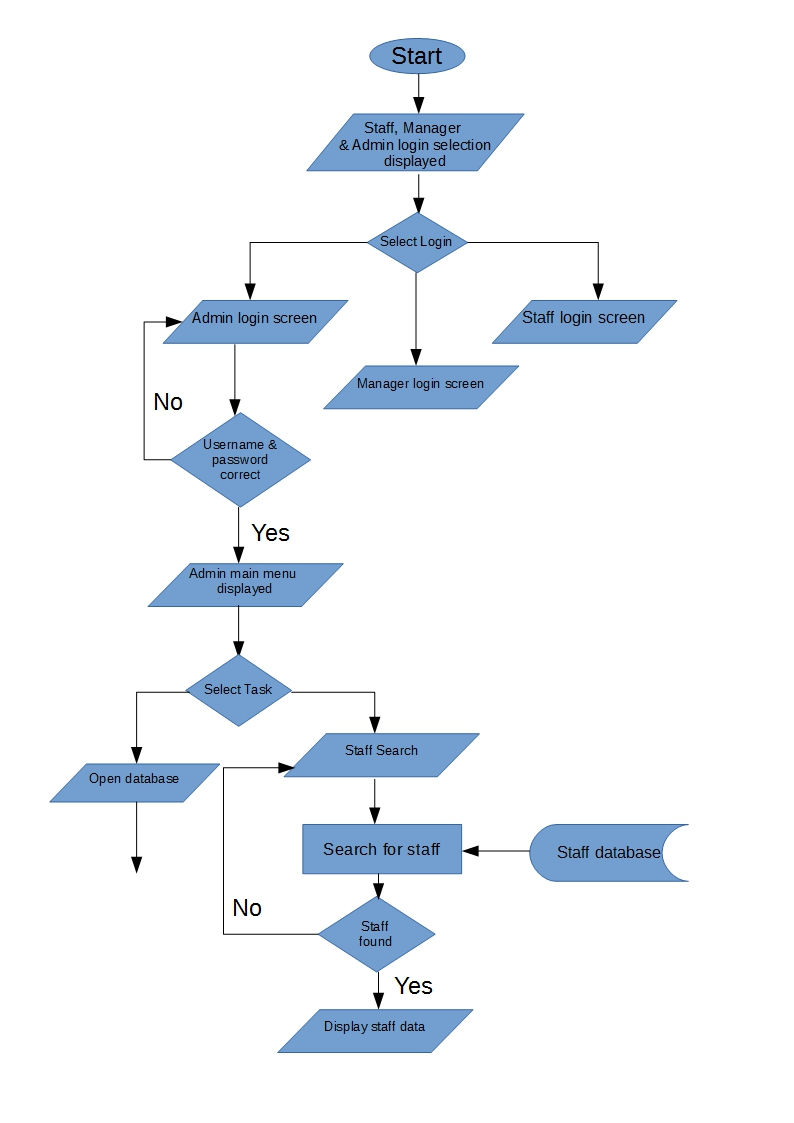
\includegraphics[width=\textwidth]{FlowchartPart1.jpg}
\end{figure}

\begin{figure}[H]
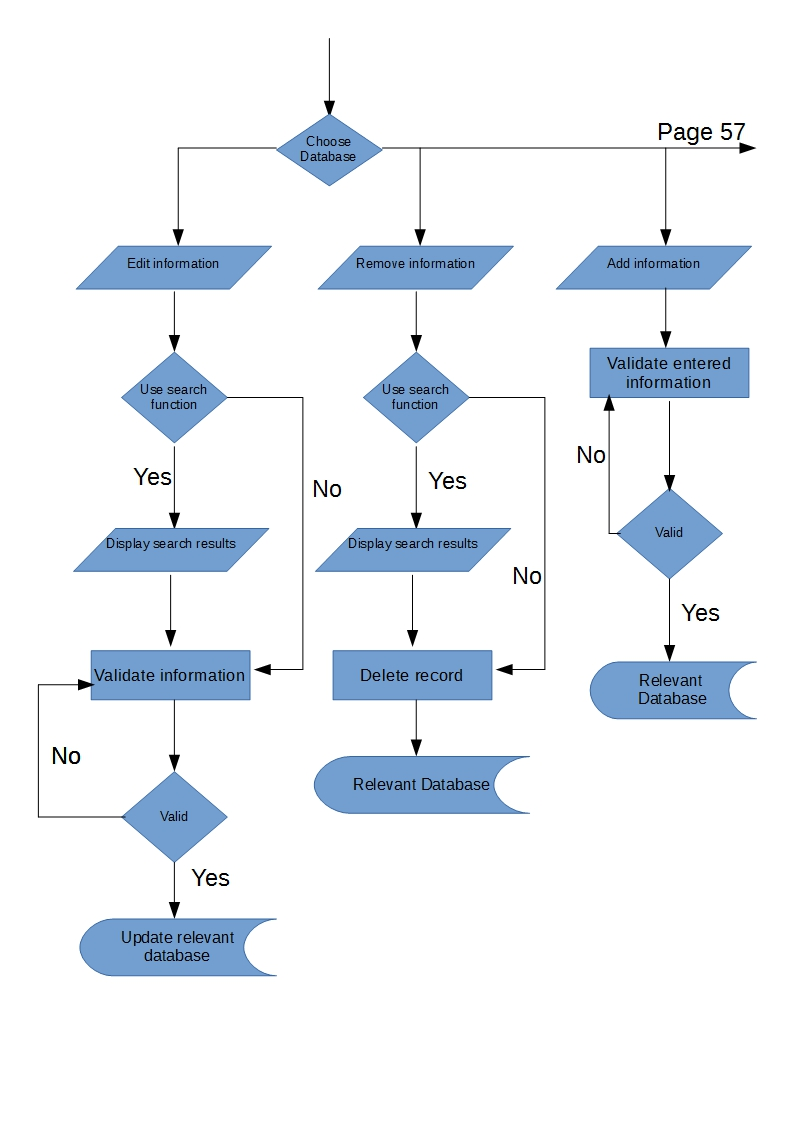
\includegraphics[width=\textwidth]{FlowchartPart2.jpg}
\end{figure}

\begin{figure}[H]
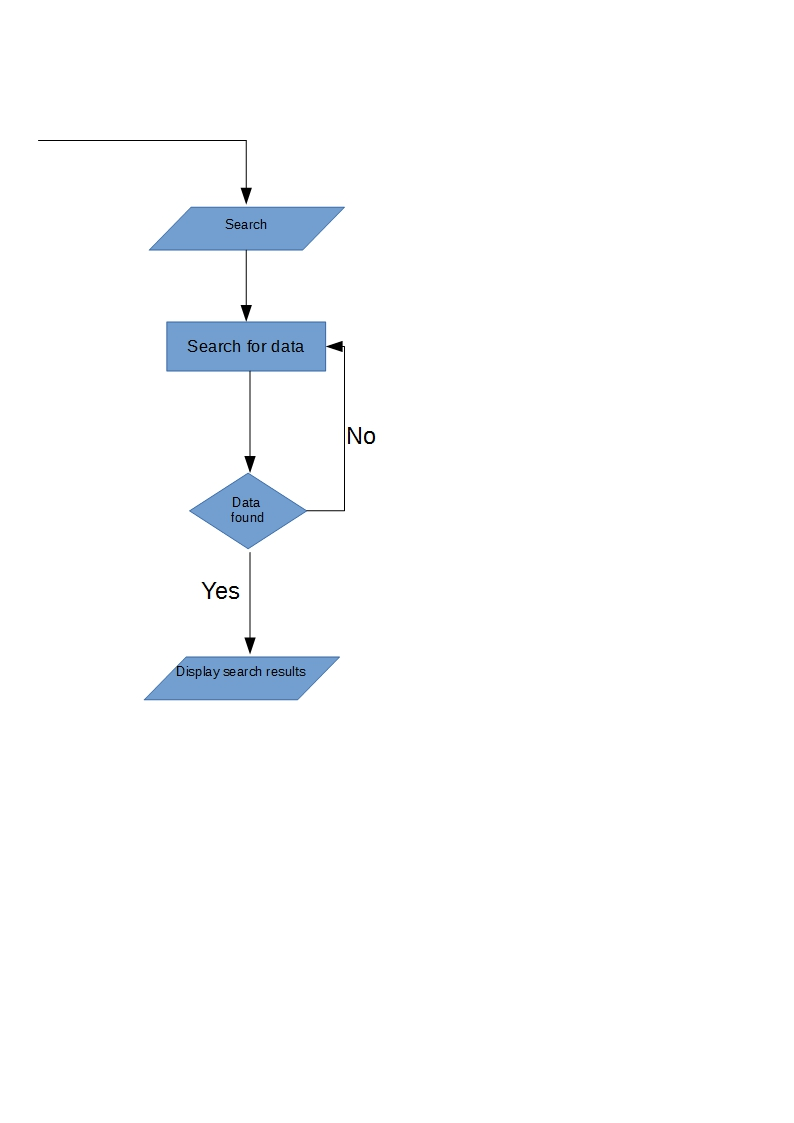
\includegraphics[width=\textwidth]{FlowchartPart3.jpg}
\end{figure}

\begin{figure}[H]
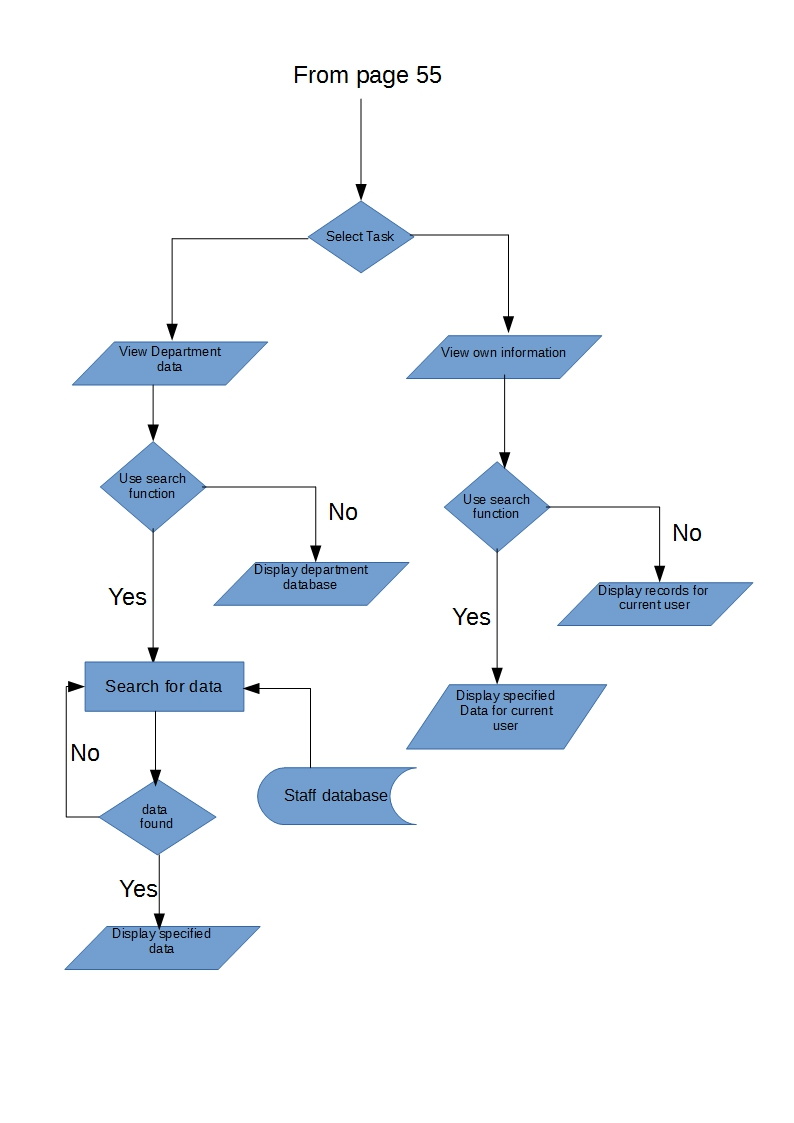
\includegraphics[width=\textwidth]{FlowchartPart4.jpg}
\end{figure}

\begin{figure}[H]
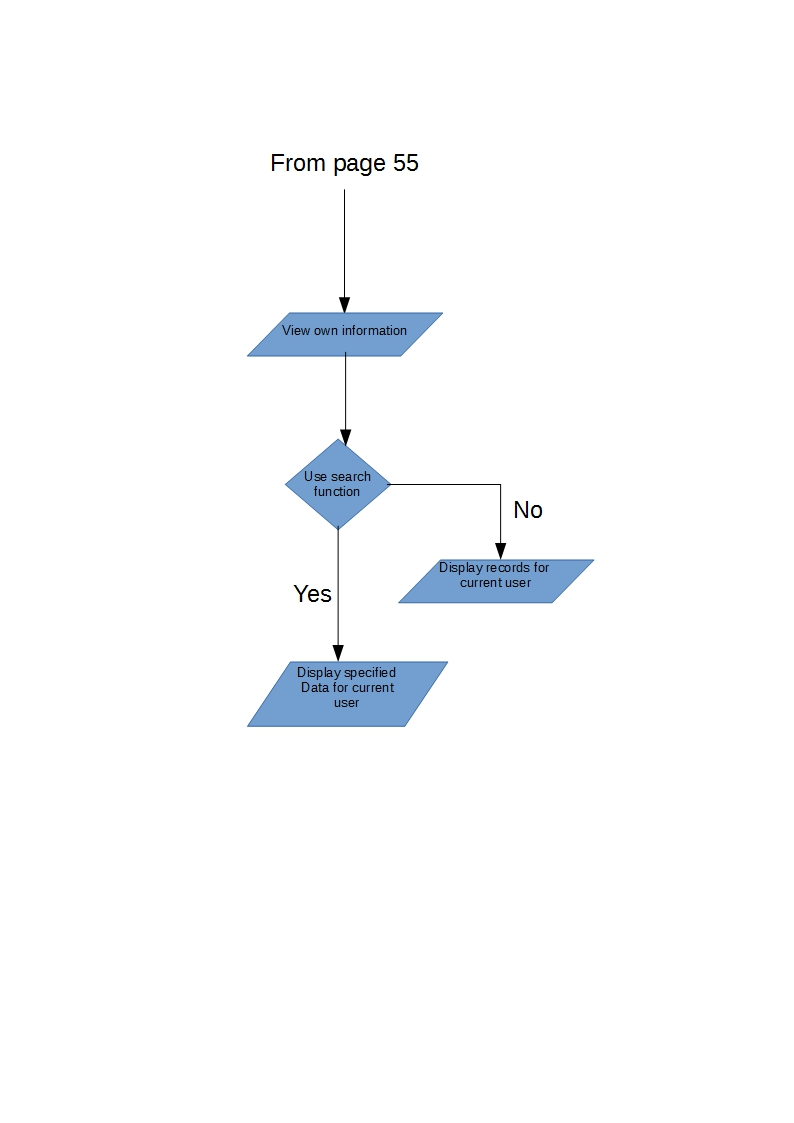
\includegraphics[width=\textwidth]{FlowchartPart5.jpg}
\end{figure}



\section{User Interface Designs}

\begin{figure}[H]
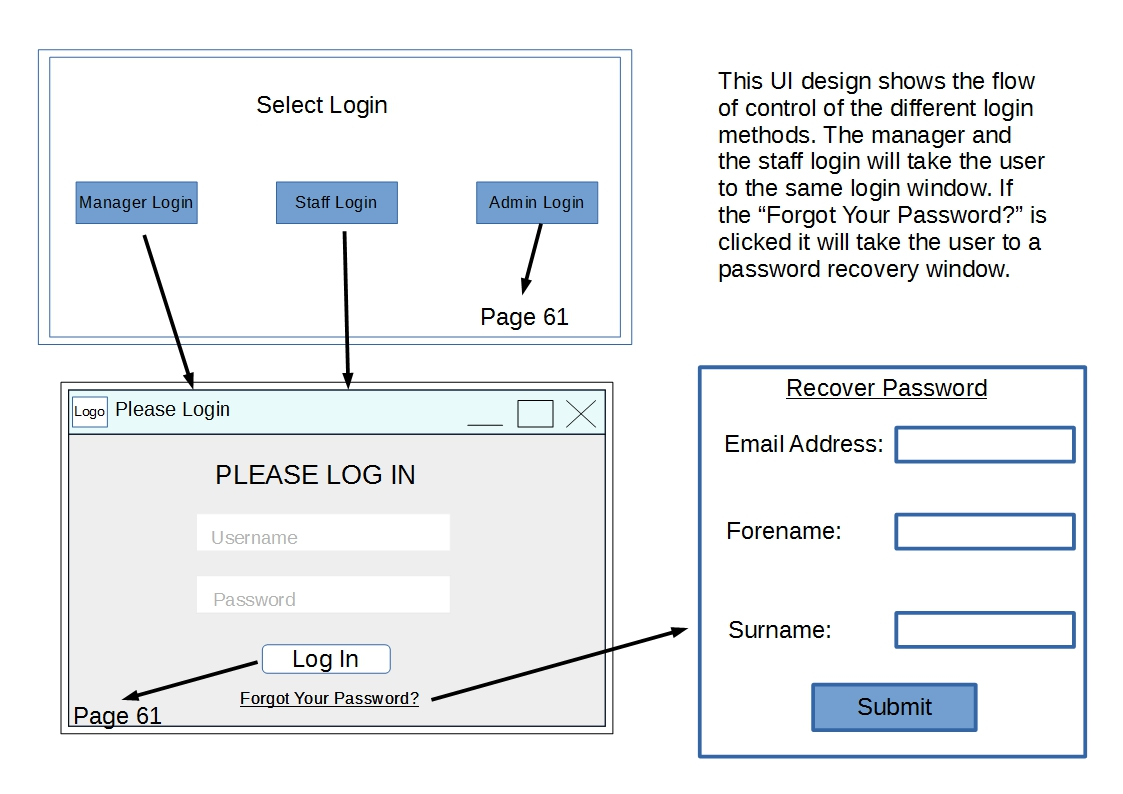
\includegraphics[width=\textwidth,angle=90]{GUI_Design1.jpg}
\caption{}
\end{figure}


\begin{figure}[H]
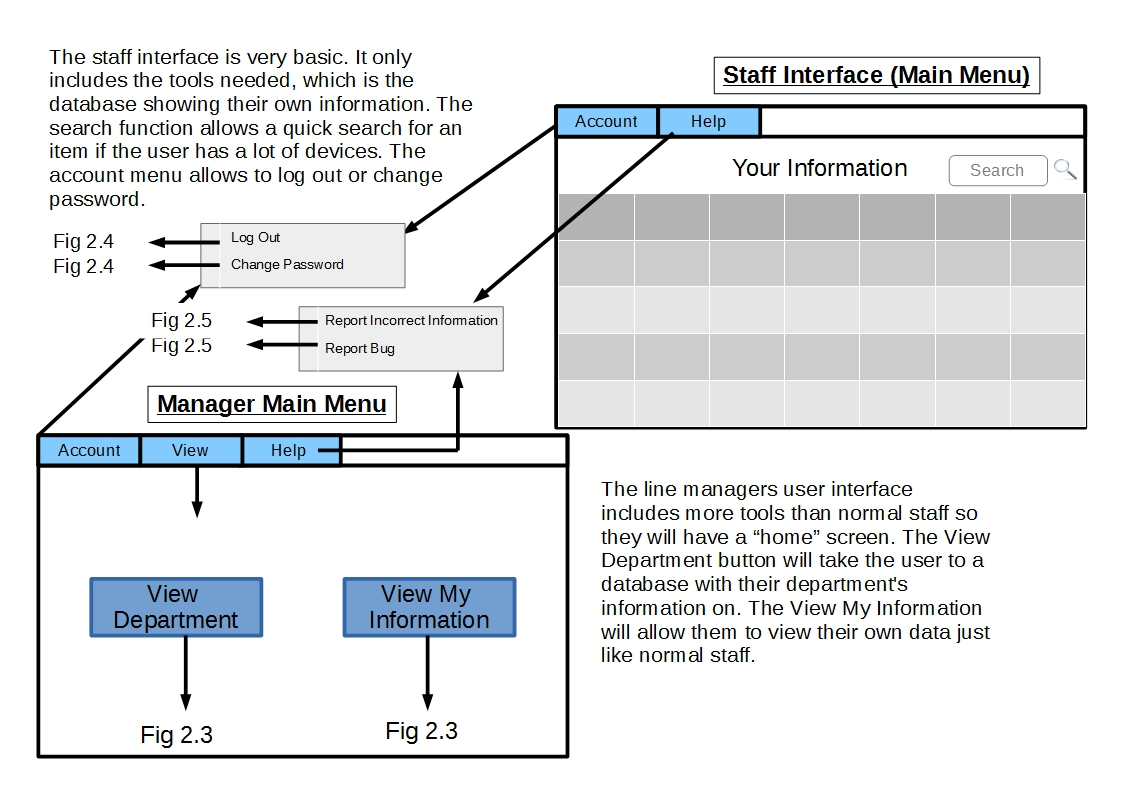
\includegraphics[width=\textwidth,angle=90]{GUI_Design2.jpg}
\caption{}
\end{figure}

\begin{figure}[H]
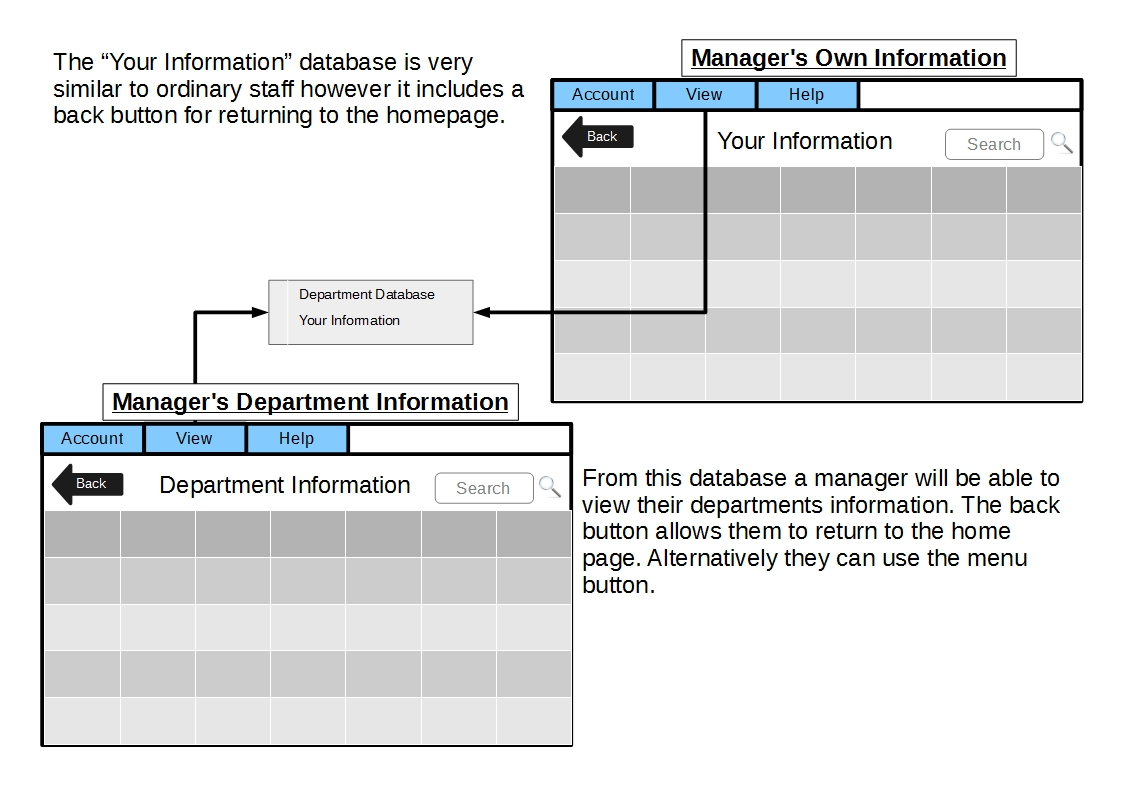
\includegraphics[width=\textwidth,angle=90]{GUI_Design3.jpg}
\caption{}
\end{figure}

\begin{figure}[H]
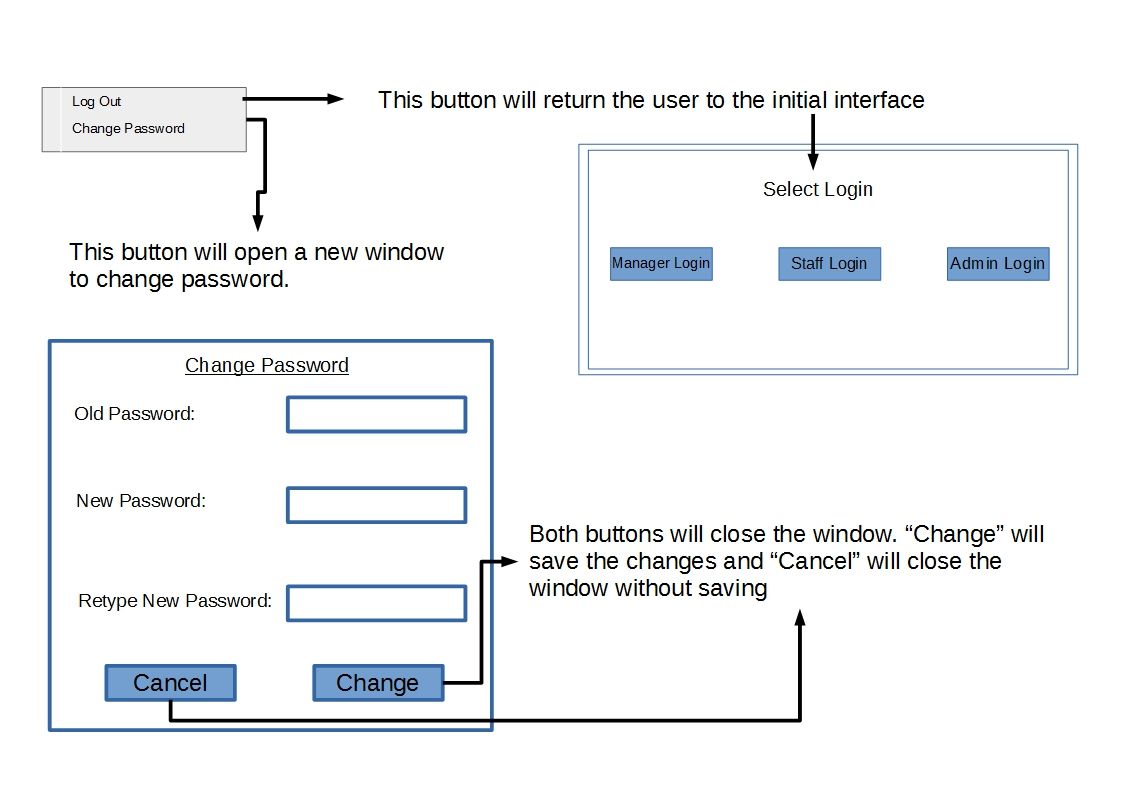
\includegraphics[width=\textwidth,angle=90]{GUI_Design4.jpg}
\caption{}
\end{figure}

\begin{figure}[H]
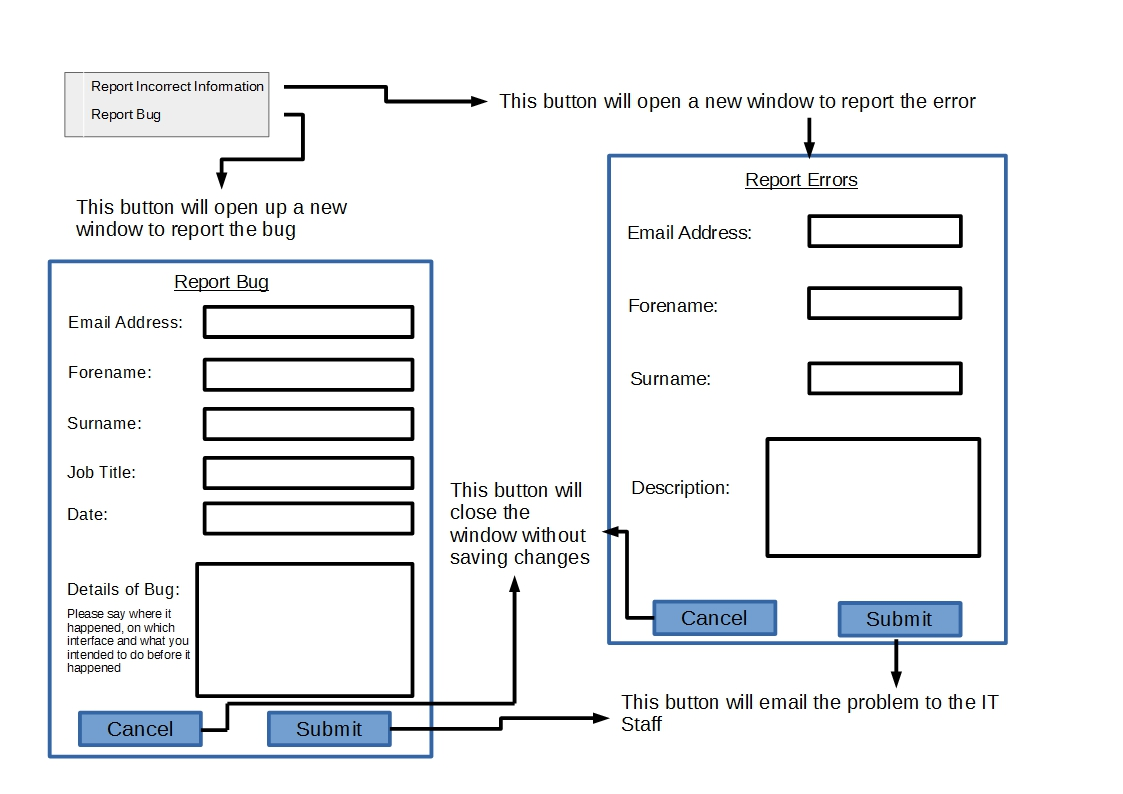
\includegraphics[width=\textwidth,angle=90]{GUI_Design5.jpg}
\caption{}
\end{figure}

\begin{figure}[H]
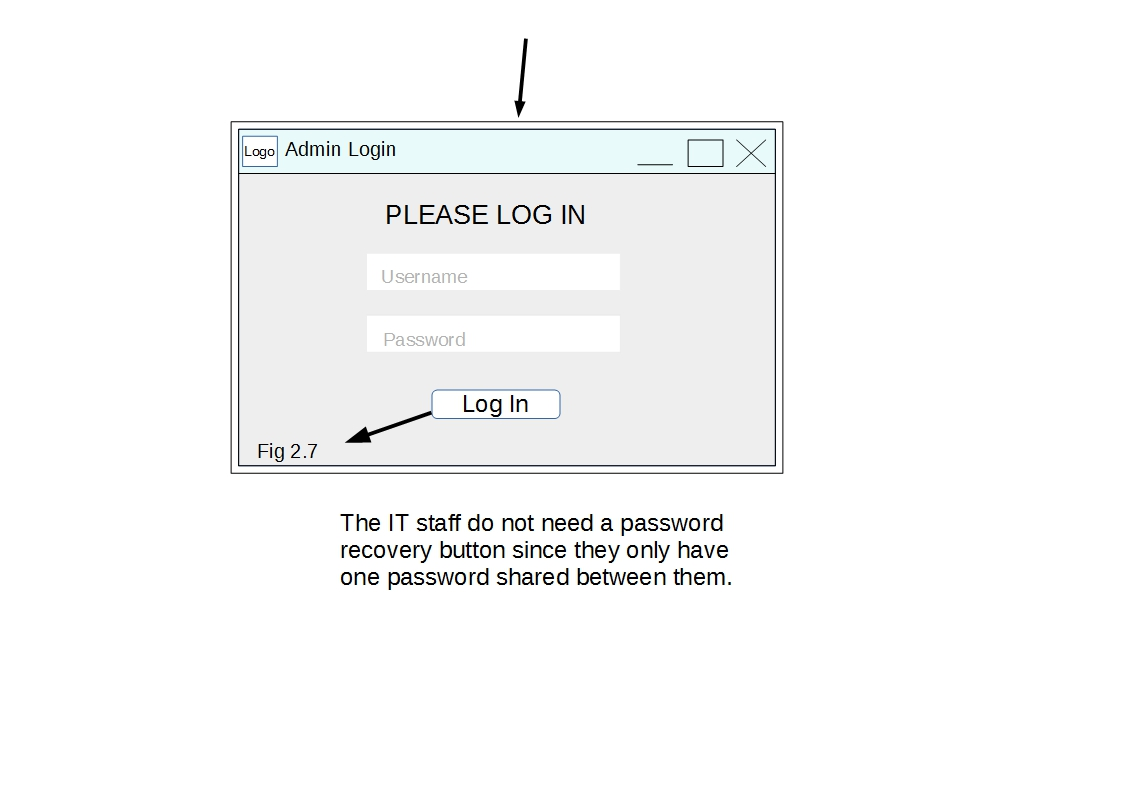
\includegraphics[width=\textwidth,angle=90]{GUI_Design6.jpg}
\caption{}
\end{figure}

\begin{figure}[H]
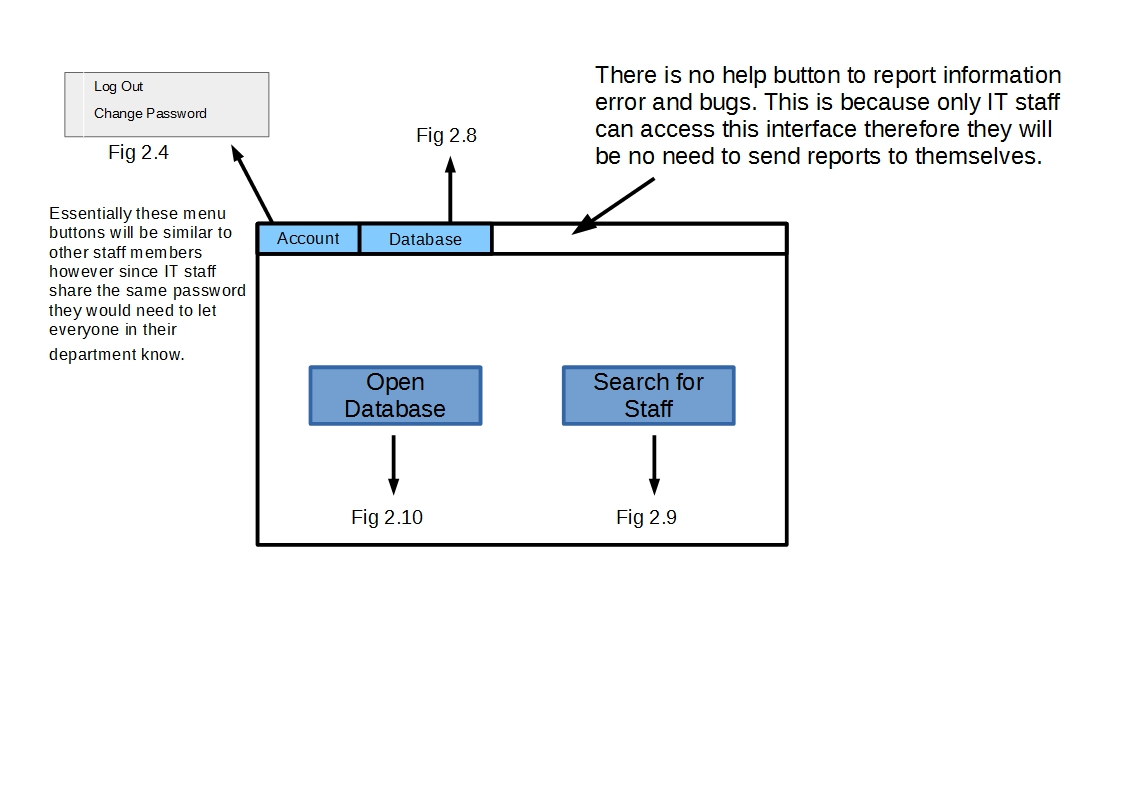
\includegraphics[width=\textwidth,angle=90]{GUI_Design7.jpg}
\caption{}
\end{figure}

\begin{figure}[H]
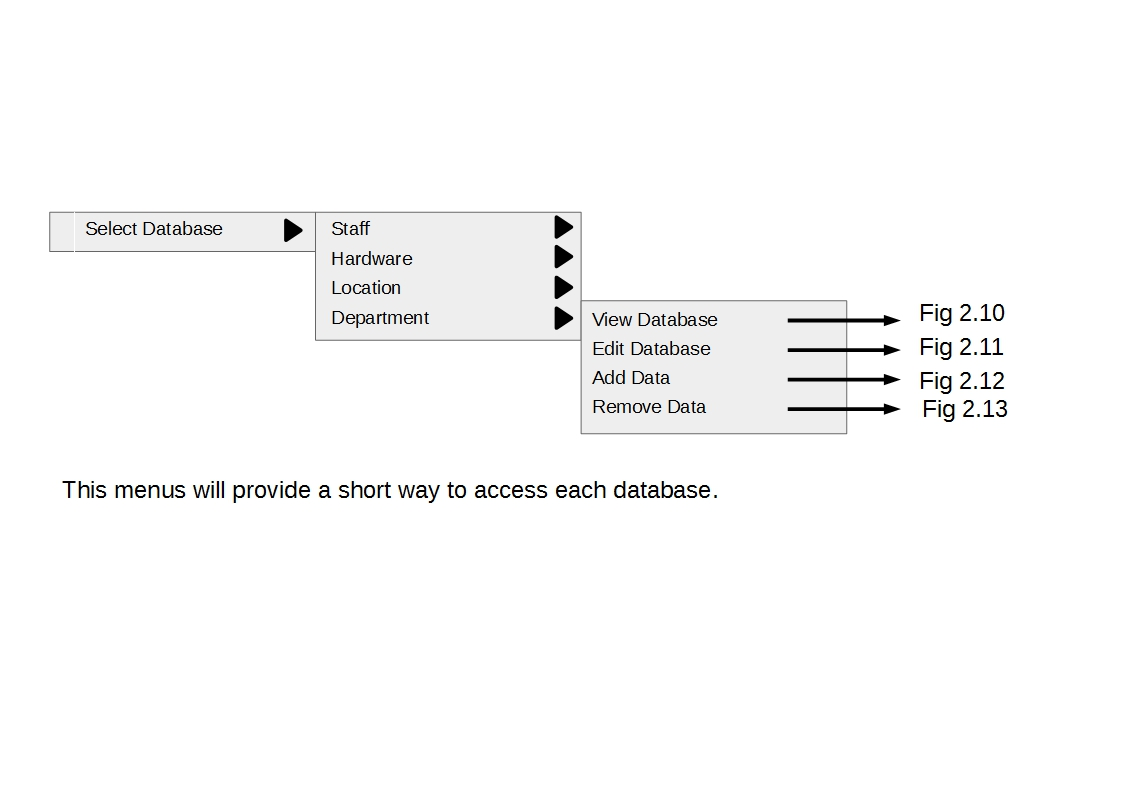
\includegraphics[width=\textwidth,angle=90]{GUI_Design8.jpg}
\caption{}
\end{figure}

\begin{figure}[H]
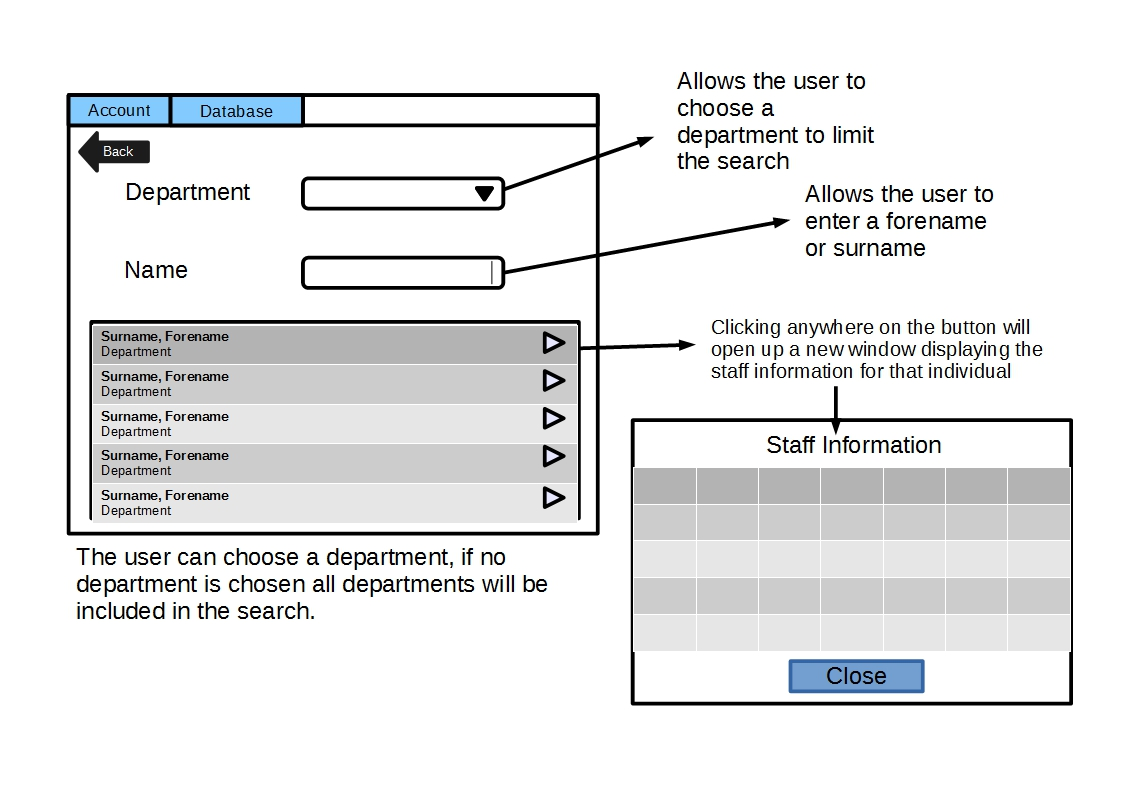
\includegraphics[width=\textwidth,angle=90]{GUI_Design9.jpg}
\caption{}
\end{figure}

\begin{figure}[H]
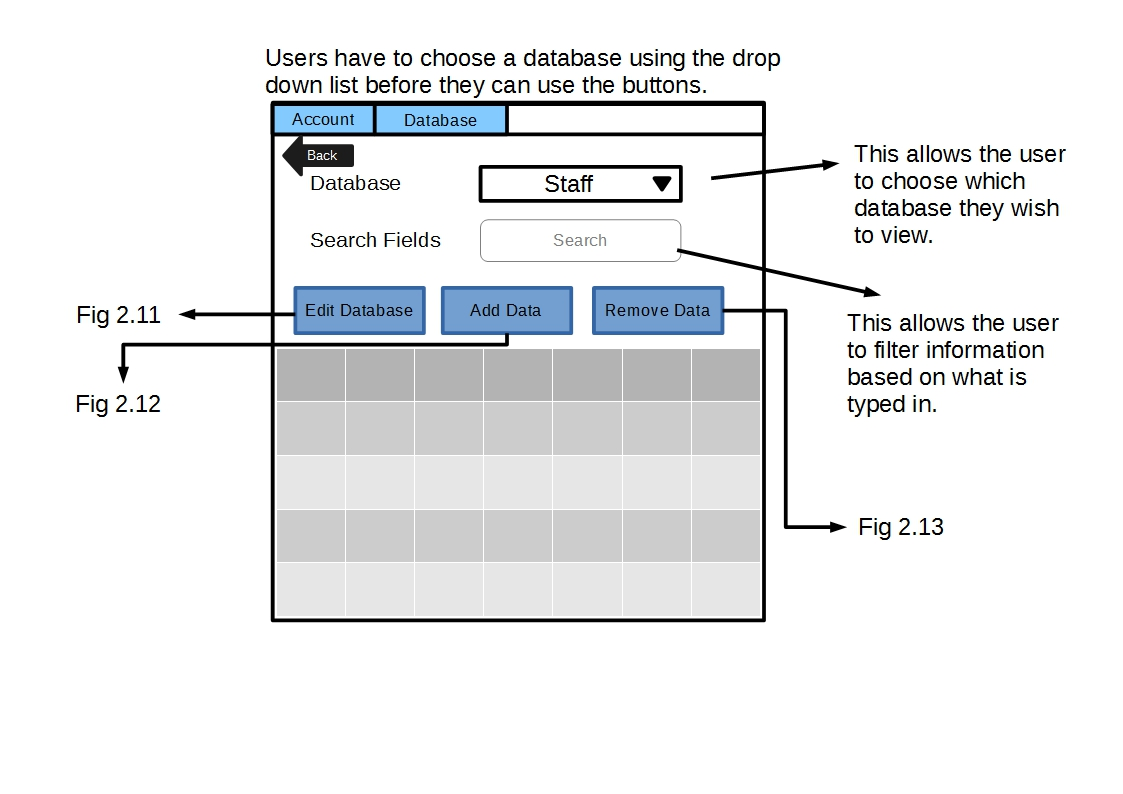
\includegraphics[width=\textwidth,angle=90]{GUI_Design10.jpg}
\caption{}
\end{figure}

\begin{figure}[H]
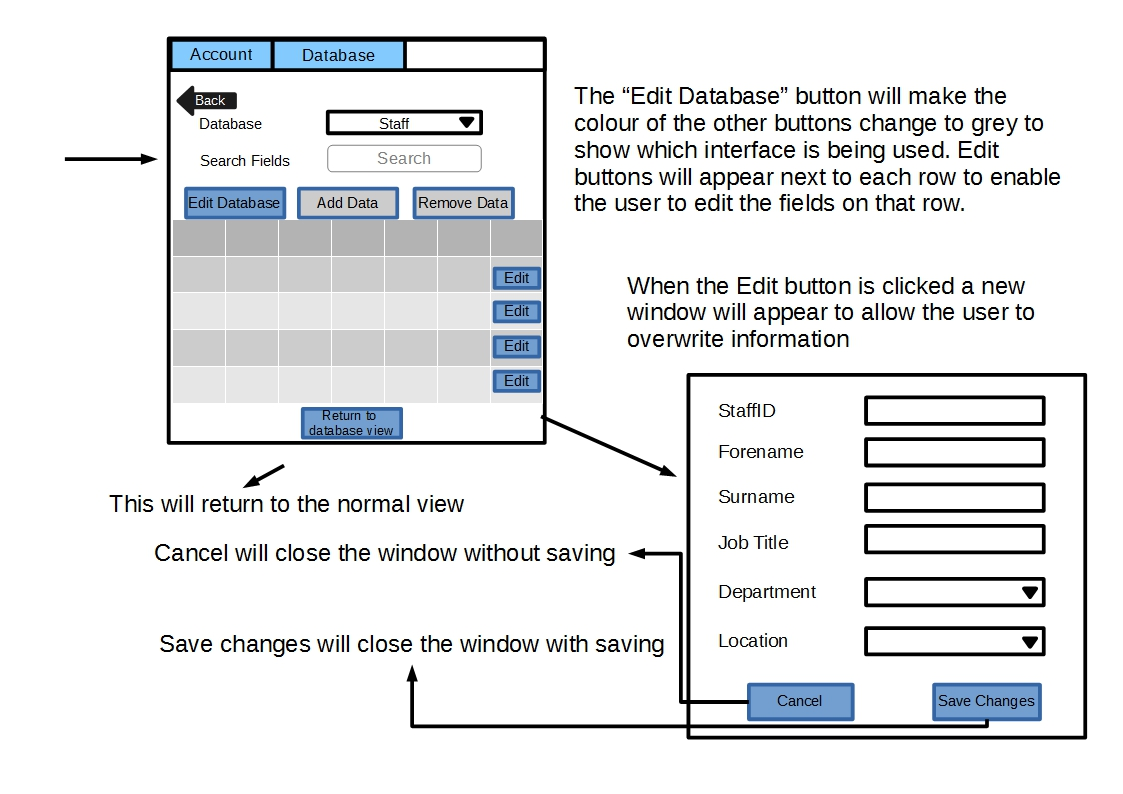
\includegraphics[width=\textwidth,angle=90]{GUI_Design11.jpg}
\caption{}
\end{figure}

\begin{figure}[H]
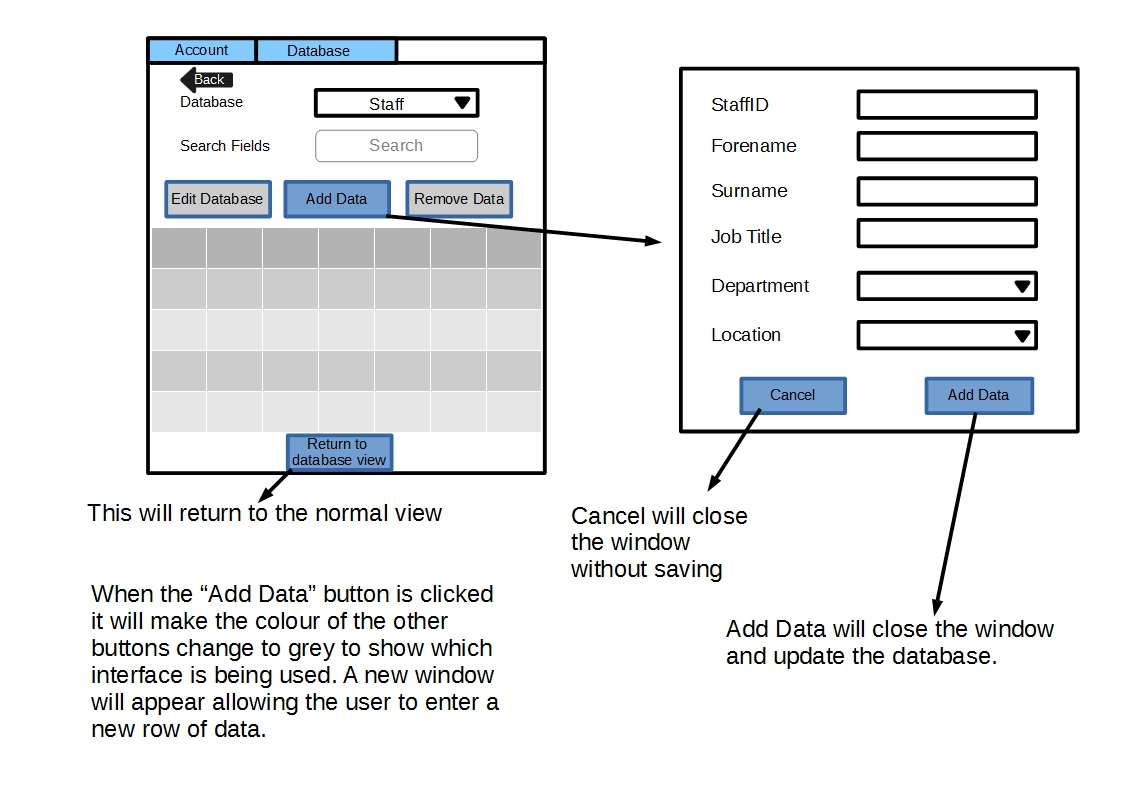
\includegraphics[width=\textwidth,angle=90]{GUI_Design12.jpg}
\caption{}
\end{figure}

\begin{figure}[H]
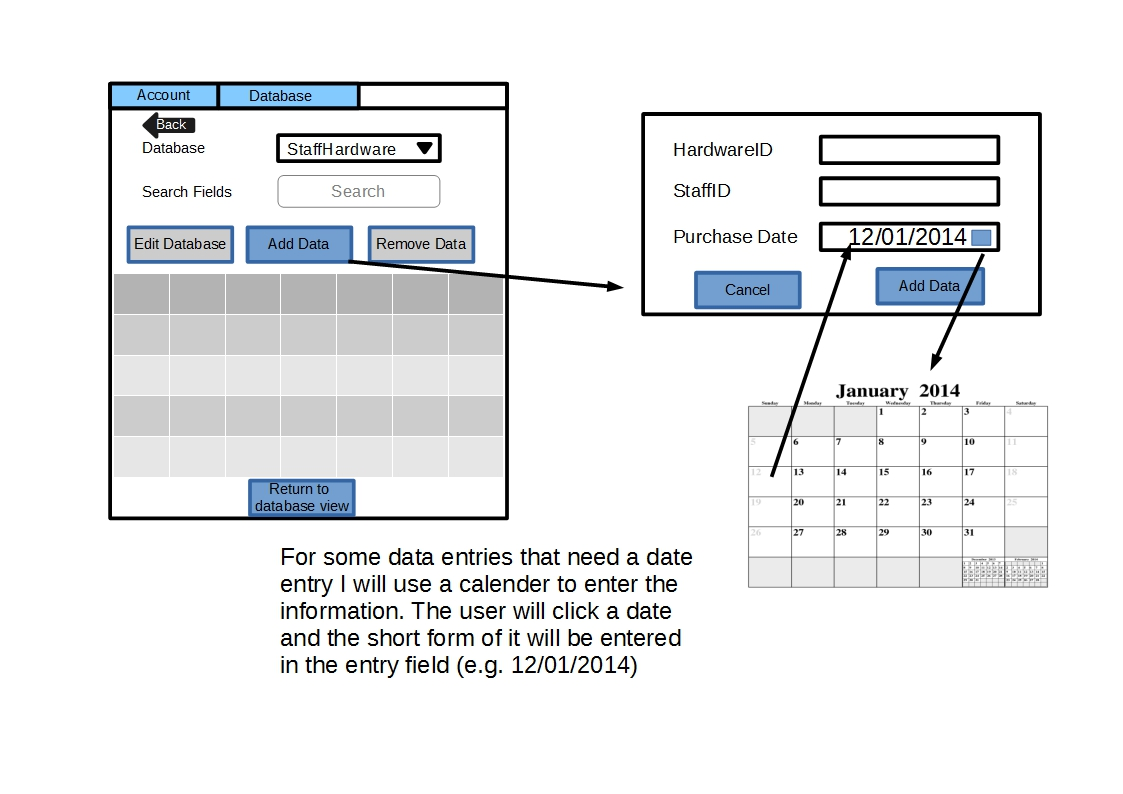
\includegraphics[width=\textwidth,angle=90]{GUI_Design13.jpg}
\caption{}
\end{figure}

\begin{figure}[H]
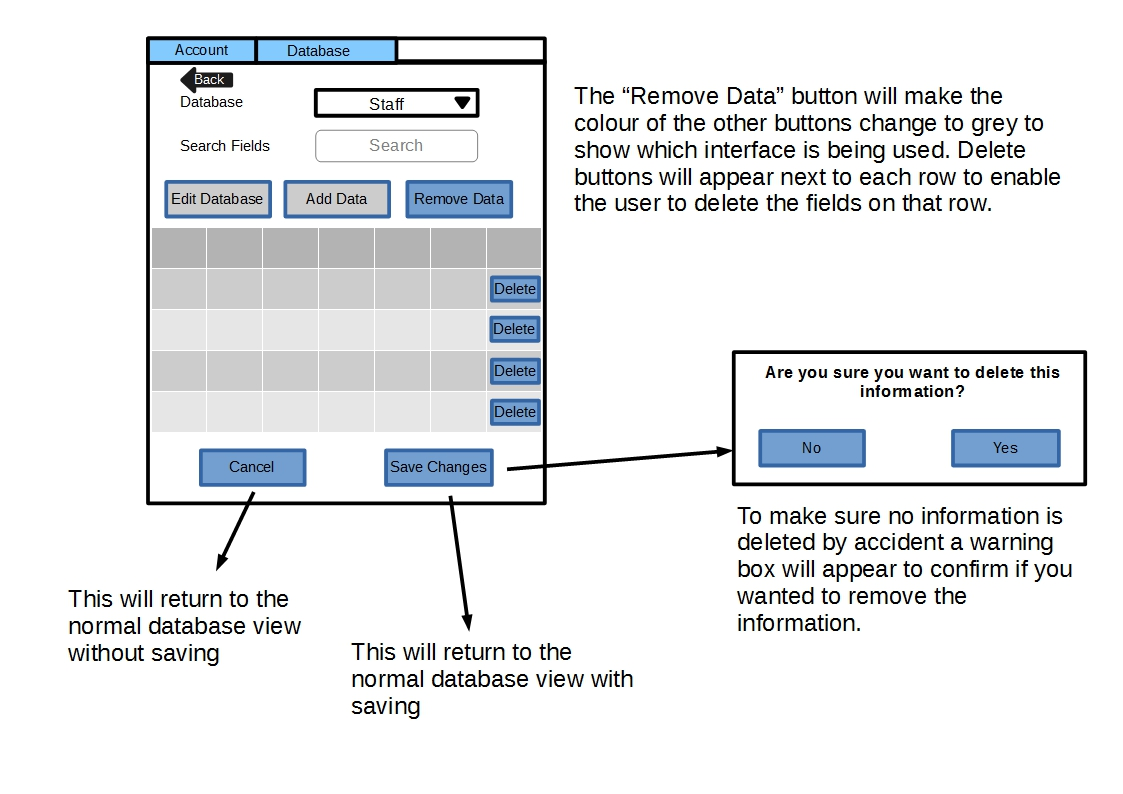
\includegraphics[width=\textwidth,angle=90]{GUI_Design14.jpg}
\caption{}
\end{figure}


\section {Hardware Specification}

The system will be stored onto a server stored in the workplace which is perfectly capable to handle the system, the specs are as followed:
\begin{itemize}
\item HP DL360
\item Windows 2003 (can run any operating system required)
\item 4TB Hard Drive
\item 16GB RAM
\item Quad Core Processor - 2.5 GHZ
\end{itemize}
The server is stored in a server room with high ventilation and fans operated 24/7. This is a huge benefit because the system can be running at all times so people can access the database. Preferably the overall model will be client-server and each user will have their own login for security. All users should connect using clients on local computers and will not directly access the server.

Users will connect to the system using their own computers at the workplace. These computers all have Windows 7 installed and run at the resolution of 1920x1080. The monitor sizes range from different locations, but the smallest would be 21" LCD monitors and the largest would be 27". These sizes will not be a problem since the application can fit on these monitors. All computers have a mouse, which is required for clicking the interface buttons, and a keyboard which is required for entering information. This system will not be developed for touch screen devices. The data for the program will be held on a hard drive inside the server that can be accessed by everyone who is connected to it. The company will not need any additional hardware to run the proposed system.

\section{Program Structure}

\subsection{Top-down design structure charts}


\begin{figure}[H]
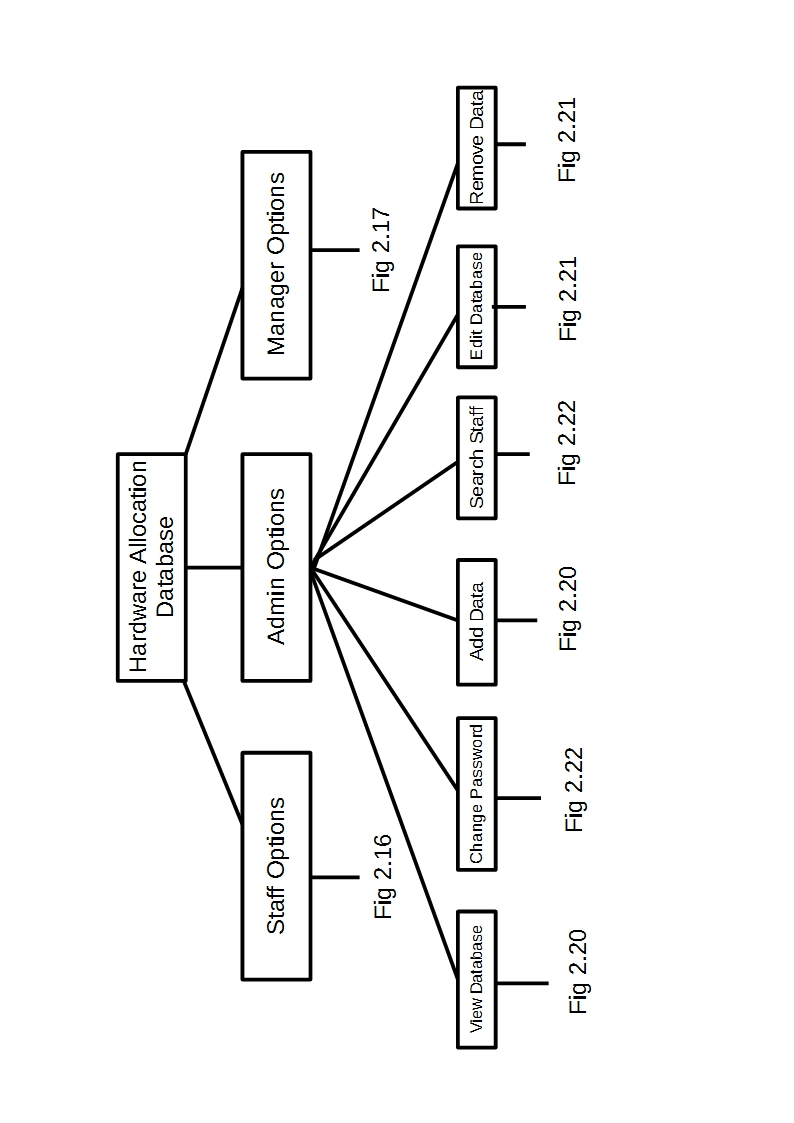
\includegraphics[width=\textwidth]{PS.jpg}
\caption{}
\end{figure}

\begin{figure}[H]
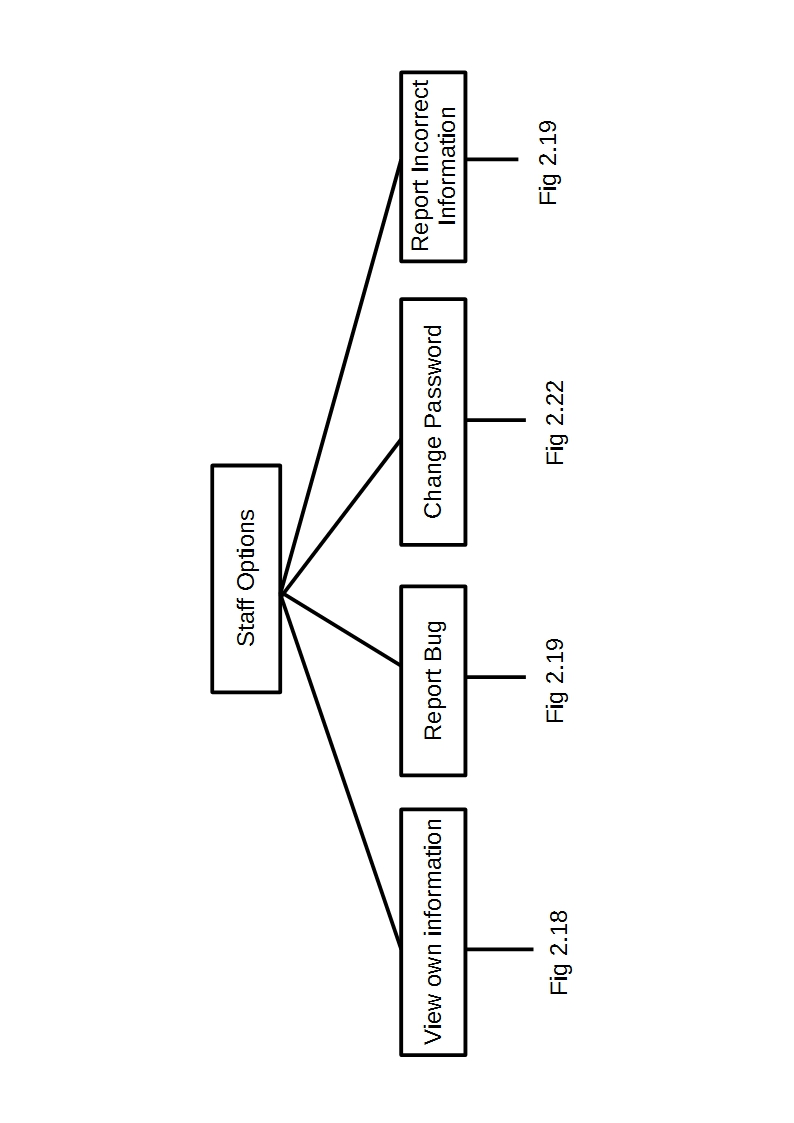
\includegraphics[width=\textwidth]{PS1.jpg}
\caption{}
\end{figure}

\begin{figure}[H]
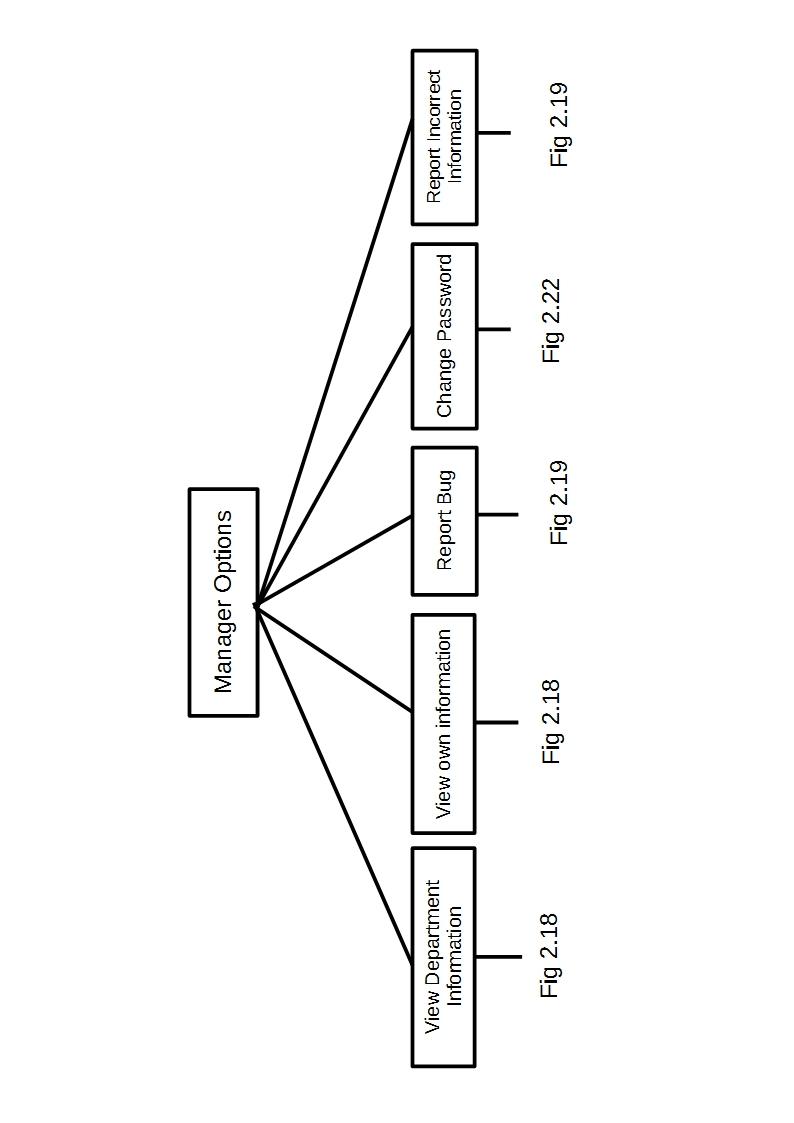
\includegraphics[width=\textwidth]{PS3.jpg}
\caption{}
\end{figure}

\begin{figure}[H]
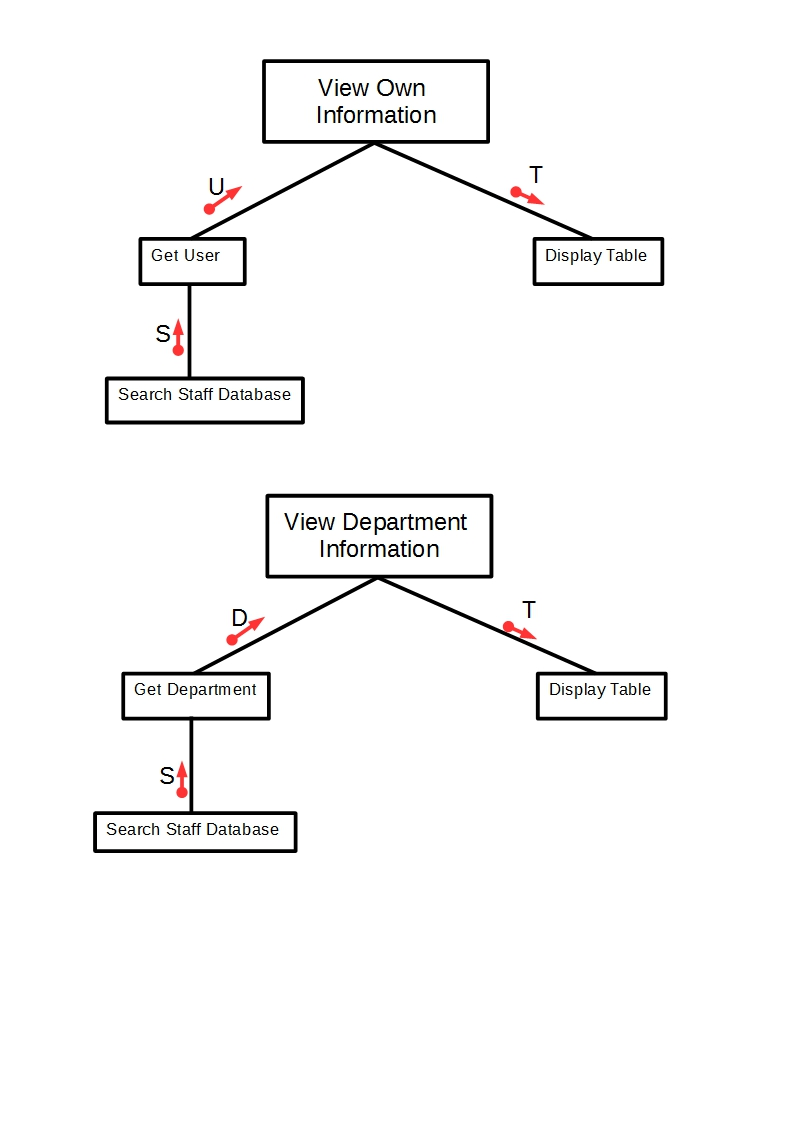
\includegraphics[width=\textwidth]{PS4.jpg}
\caption{}
\end{figure}

\begin{figure}[H]
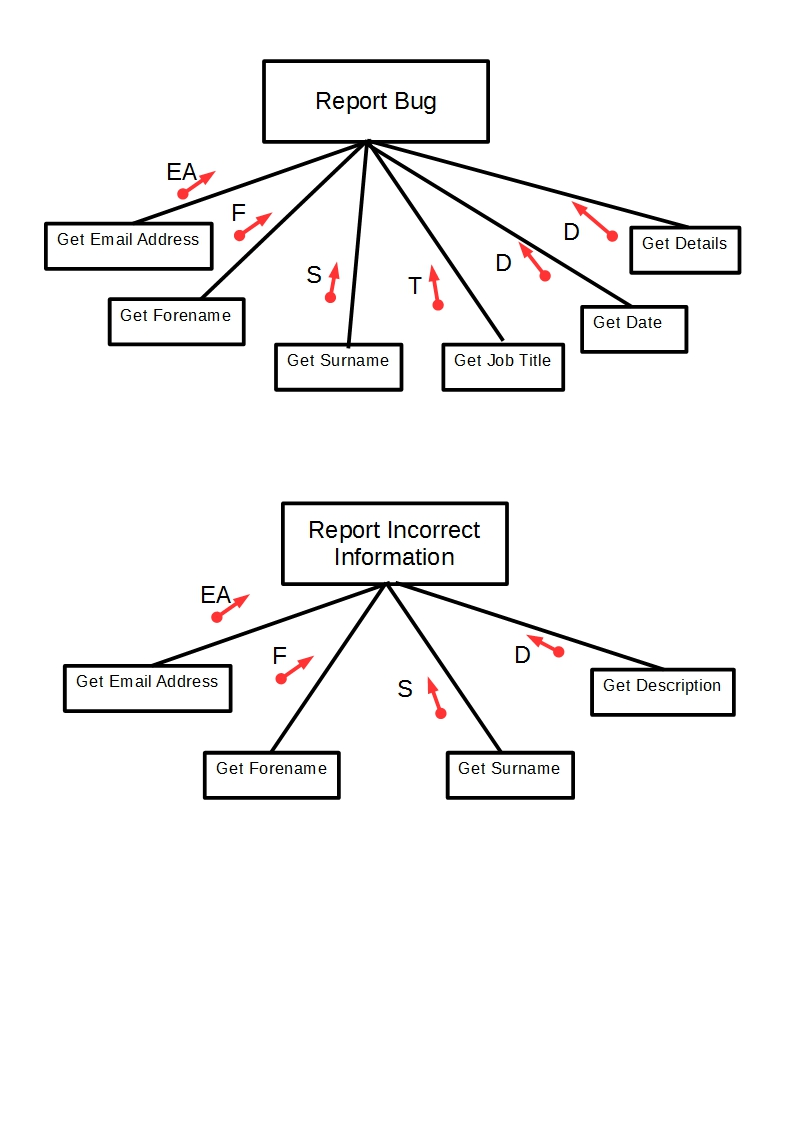
\includegraphics[width=\textwidth]{PS5.jpg}
\caption{}
\end{figure}

\begin{figure}[H]
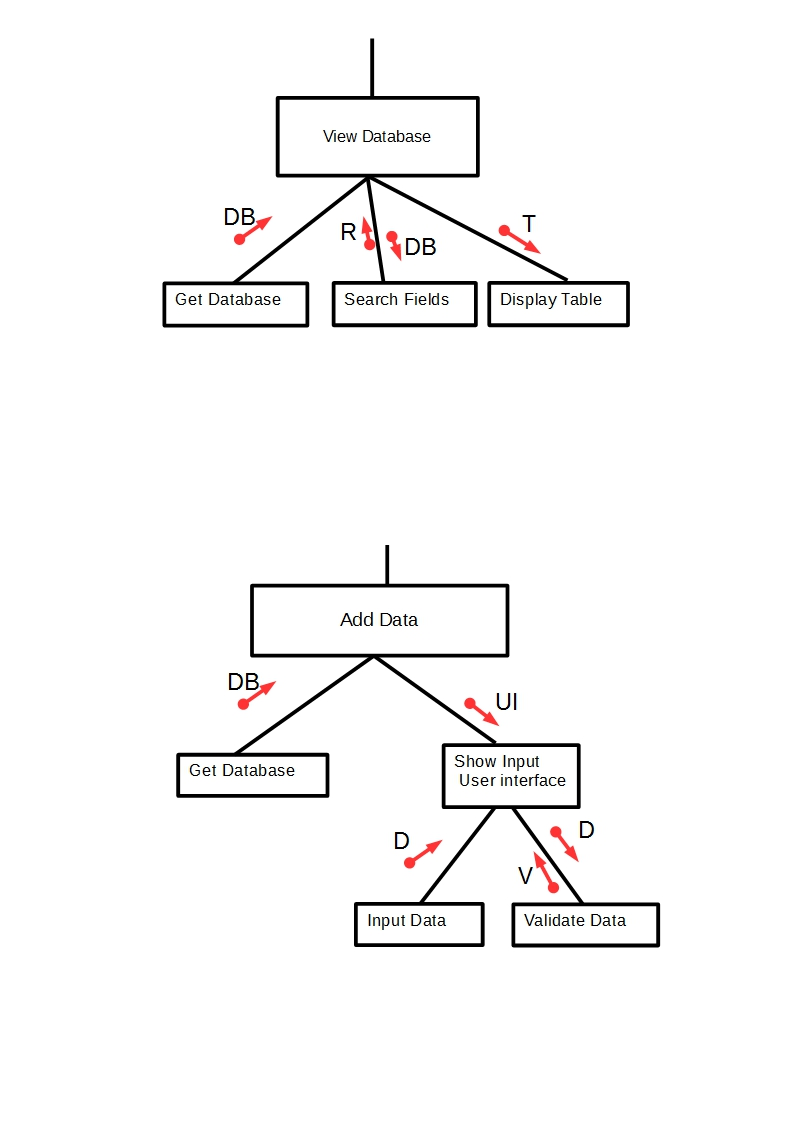
\includegraphics[width=\textwidth]{PS6.jpg}
\caption{}
\end{figure}

\begin{figure}[H]
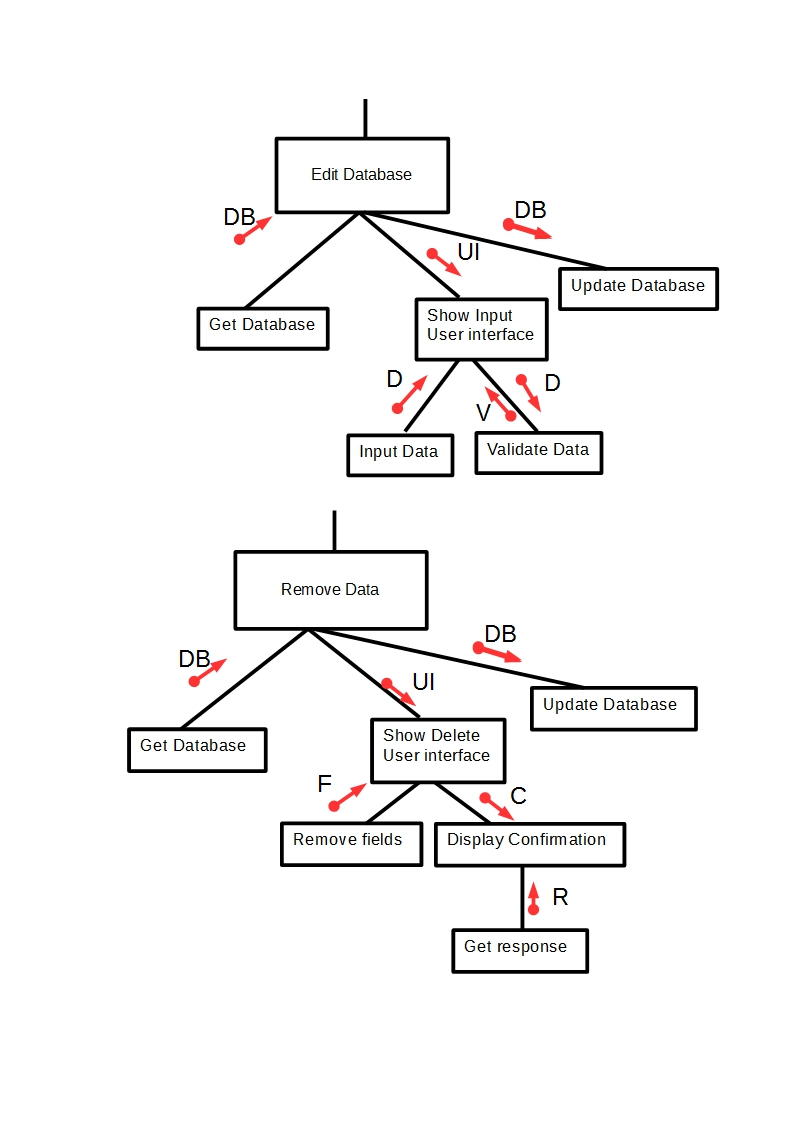
\includegraphics[width=\textwidth]{PS7.jpg}
\caption{}
\end{figure}
\begin{figure}[H]
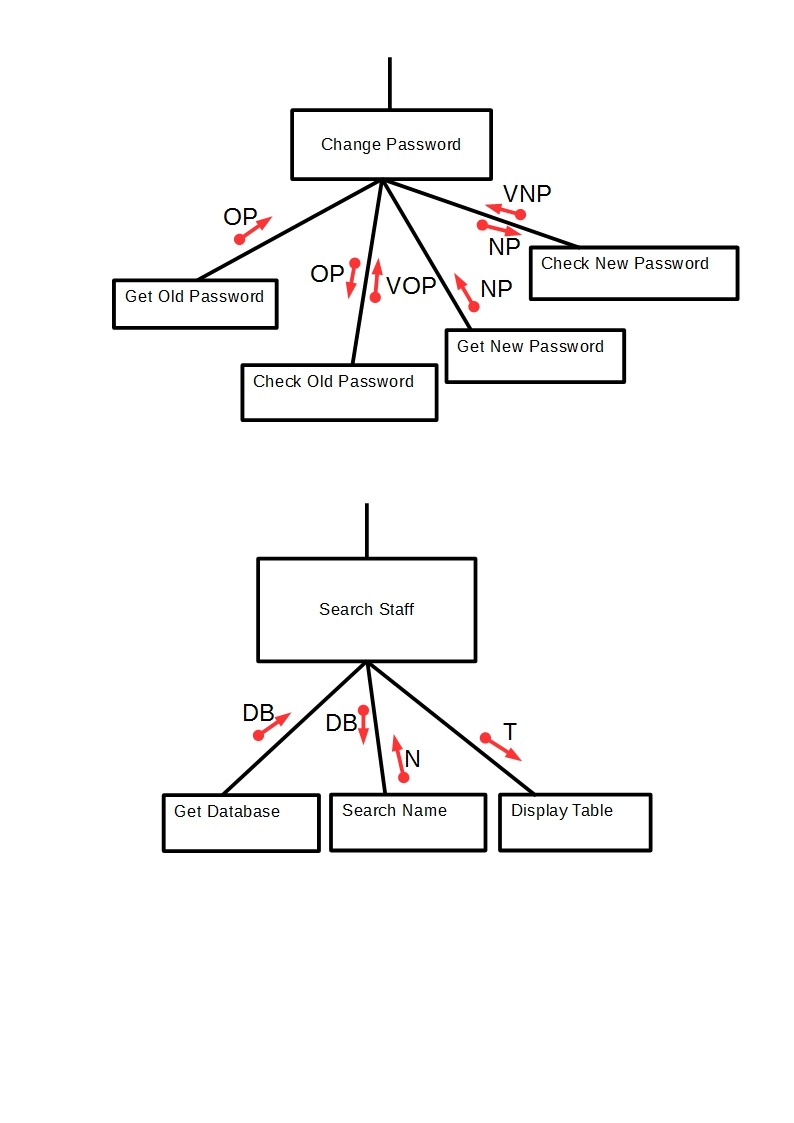
\includegraphics[width=\textwidth]{PS8.jpg}
\caption{}
\end{figure}

\subsection{Algorithms in pseudo-code for each data transformation process}


\begin{algorithm}[H]
\begin{algorithmic}
\Function {SearchStaff}{FirstName,LastName,Department}
\State Count: Integer
\State$Count \leftarrow 0$
\State ARRAY StaffList: Integer[$\infty$]
\State CONNECT to staff database
\State {StaffMembers $\leftarrow$ SEARCH staff database for staff}
\For {staff}  {StaffMembers}
	\If{staff.FirstName = FirstName AND staff.LastName = LastName AND staff.Department = Department}
		\State$StaffList[Count] \leftarrow staff$
		\EndIf
	\State$Count \leftarrow Count + 1$
	\EndFor
\State RETURN StaffList
\EndFunction
\end{algorithmic}
\end{algorithm}

\begin{algorithm}[H]
\begin{algorithmic}
\Function {ValidateOldPassword}{OldPassword, CheckOldPassword}
\State ValidPassword: Boolean
\State$ValidPassword \leftarrow FALSE$
\If{OldPassword = CheckOldPassword}
	\State$ValidPassword \leftarrow TRUE$
	\EndIf
\State RETURN ValidPassword
\EndFunction
\end{algorithmic}
\end{algorithm}

\begin{algorithm}[H]
\begin{algorithmic}
\Function {ValidateNewPassword}{NewPassword}
\State ValidPassword: Boolean
\State$ValidPassword \leftarrow FALSE$
\If{length of 20 $\geq $NewPassword $\geq$ 6}
	\State $ValidPassword \leftarrow TRUE$
\EndIf
\State RETURN ValidPassword
\EndFunction
\end{algorithmic}
\end{algorithm}

\begin{algorithm}[H]
\begin{algorithmic}
\Function {UsernameValid}{UsernameInput}
\State ValidUsername: Boolean
\State$ValidUsername \leftarrow FALSE$
\If{length of 12 $\geq $UsernameInput $\geq$ 3}
	\State $ValidUsername \leftarrow TRUE$
\EndIf
\State RETURN ValidUsername
\EndFunction
\end{algorithmic}
\end{algorithm}

\begin{algorithm}[H]
\begin{algorithmic}
\Function {AddStaff}{FirstName, LastName, JobTitle, LocationID, DepartmentID}
\State DepartmenIDFound: Boolean
\State LocationIDFound: Boolean
\State CONNECT to staff database
\State CONNECT to location database
\State CONNECT to department database
\State ARRAY LocationList: Integer [$\infty$]
\State ARRAY DepartmentList: Integer [$\infty$]
\State DepartmentList $\leftarrow$ SEARCH department database for DepartmentID
\For {department} {DepartmentList}
	\If {DepartmentID = department}
		\State DepartmentIDFound $\leftarrow$ TRUE
	\EndIf
\EndFor
\State LocationList $\leftarrow$ SEARCH location database for LocationID
\For {Location} {LocationList}
	\If {LocationID = location}
		\State LocationIDFound $\leftarrow$ TRUE
	\EndIf
\EndFor

\If {DepartmentID AND LocationID}
	\State ADD staff database FirstName = FirstName, LastName = LastName, DepartmentID = DepartmentID, LocationID = LocationID
\EndIf

\EndFunction
\end{algorithmic}
\end{algorithm}

\begin{algorithm}[H]
\begin{algorithmic}
\Function {RemoveData}{StaffID}
\State StaffIDFound: Boolean
\State CONNECT to staff database
\State ARRAY StaffList: Integer [$\infty$]
\State StaffList $\leftarrow$ SEARCH staff database for StaffID
\For {staff} {StaffList}
	\If {StaffID = staff}
		\State StaffIDFound $\leftarrow$ TRUE
	\EndIf
\EndFor
\If {StaffIDFound}
	\State REMOVE staff database FirstName = FirstName, LastName = LastName, DepartmentID = DepartmentID, LocationID = LocationID
\EndIf

\EndFunction
\end{algorithmic}
\end{algorithm}

\subsection{Object Diagrams}

\begin{figure}[H]
\hspace*{-1.3cm}
\vspace*{-1cm}
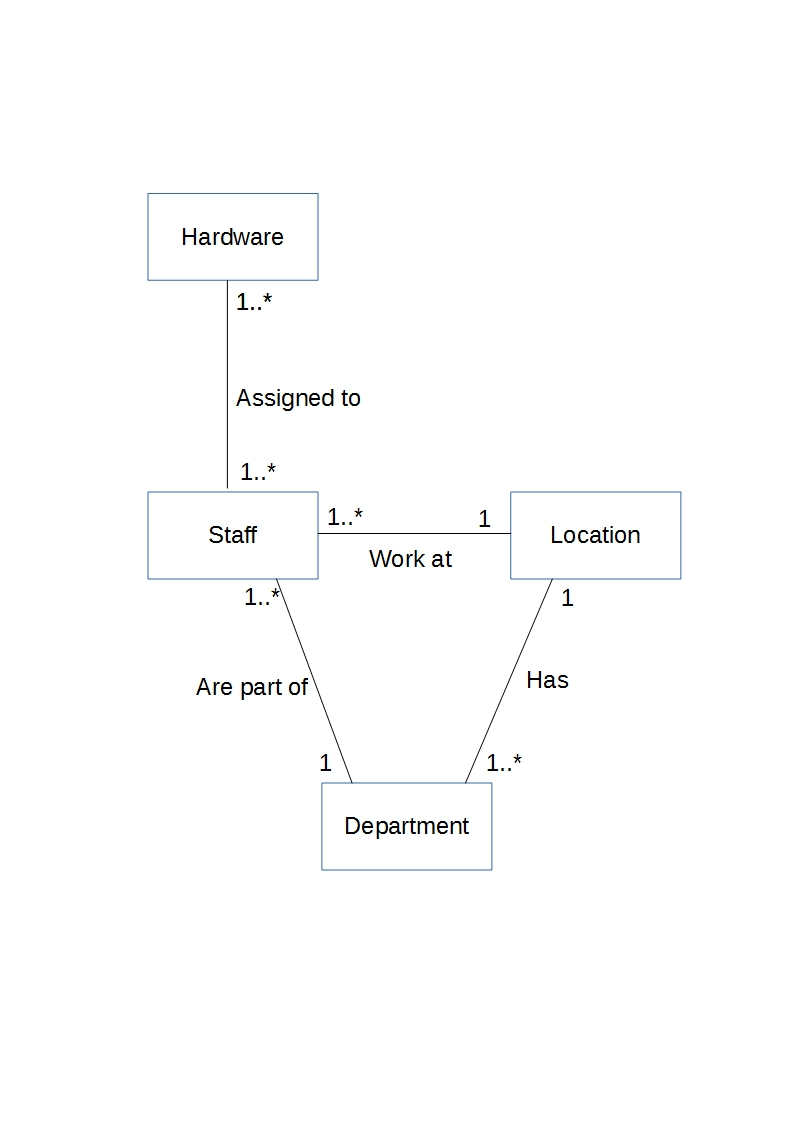
\includegraphics[width=1\textwidth]{RelationshipDiagram.jpg}
\caption{The relationship diagram shows how staff own many hardware devices. The staff work at one work location and that location has many different departments. Many staff are part of one department. } \label{Relationship Diagrams}
\end{figure}

\subsection{Class Definitions}

\begin{figure}[H]
\hspace*{-1.3cm}
\vspace*{-1cm}
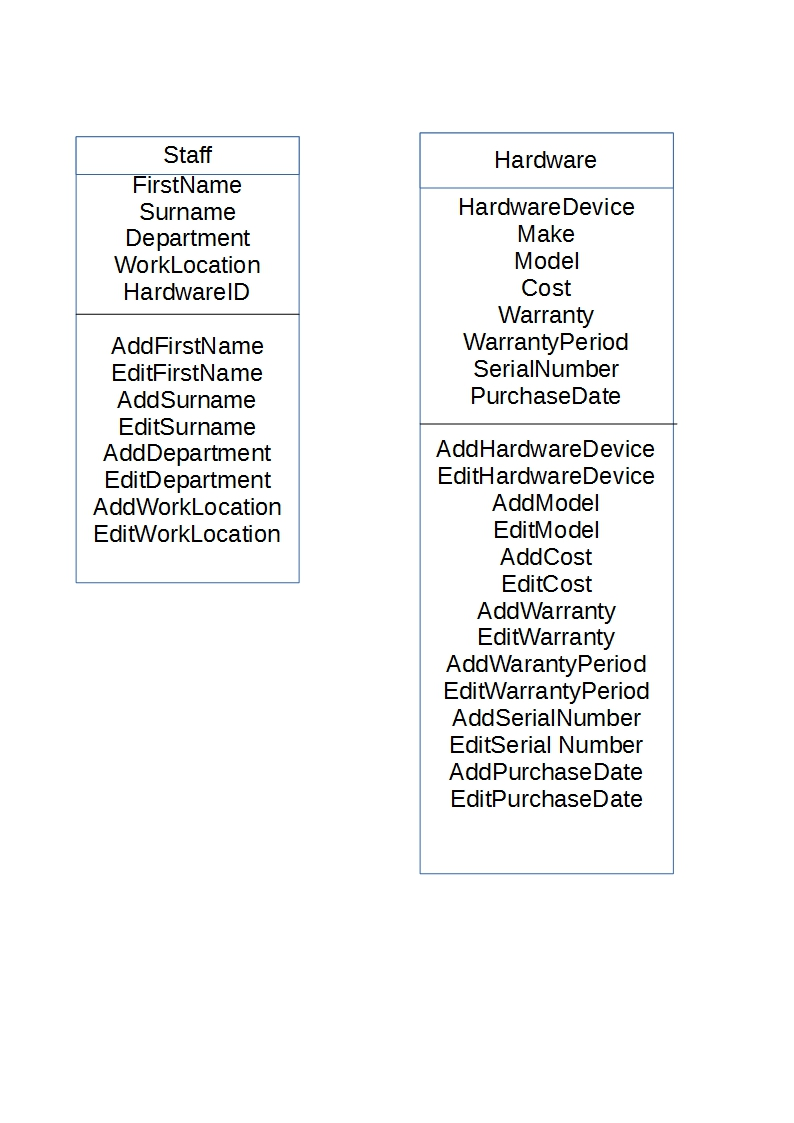
\includegraphics[width=1\textwidth]{ClassDefinitions.jpg}
\caption{The class definitions show the attributes and methods for each class. The staff class will hold unique IDs from the other classes to make the relationship.} \label{Class Definitions}
\end{figure}

\section{Prototyping}

Prototyping is going to be very helpful as I can test out different parts of my program and see if they will function the way I would like them to or not.

\

\underline {\textbf{The Login Window}}

\

I made a prototype for the login window to get to grips with how to validate information and use colours. The validation tells the user that the username has to be 5 digits (cannot include letters). The password is the part of the prototype that was focused on most since it is important that it is censored out. The password cannot be copied and pasted anywhere (to add security).

\begin{figure}[H]
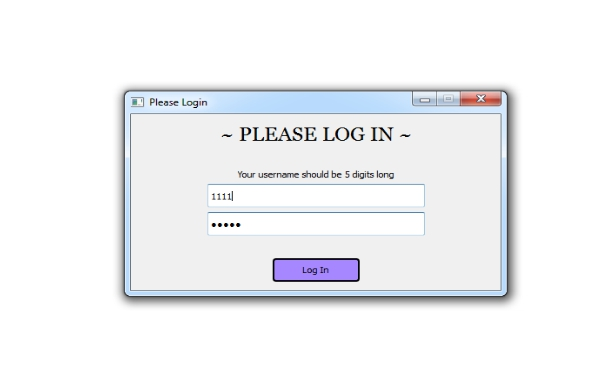
\includegraphics[width=\textwidth]{LoginWindow.jpg}
\caption{Login Window}
\end{figure}

\newpage

The login window will have a system that tells the user a correct format has been added (A tick will be placed next to the box).
\begin{figure}[H]
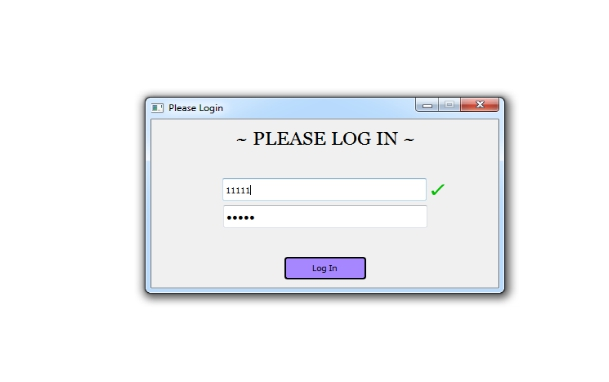
\includegraphics[width=\textwidth]{LoginWindow2.jpg}
\caption{Login Window}
\end{figure}

\newpage

\underline {\textbf{The Calender}}

\

Another prototype I made was a calender. This will be used when inputting dates. I chose to design this to see how difficult it would be to track when someone clicks a date on the calender and display the date that was clicked. For example below shows a label at the bottom displaying what date has been selected.

\begin{figure}[H]
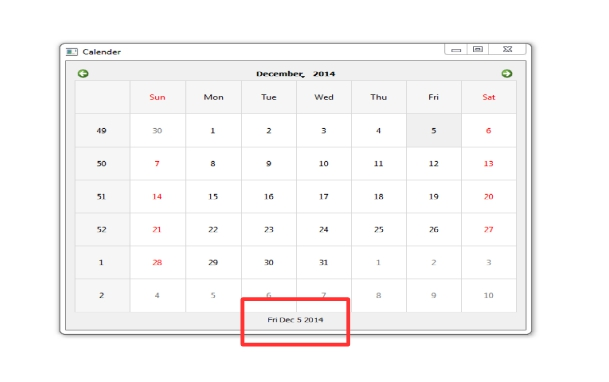
\includegraphics[width=\textwidth]{Calender.jpg}
\caption{Login Window}
\end{figure}


\section{Definition of Data Requirements}

\subsection{Identification of all data input items}

\begin{itemize}
\item Username
\item Password
\item Email Address
\item First Name
\item Surname
\item Job Title
\item Date (On Bug Report)
\item Details of Bug Reports
\item Details of Information Errors
\item Department
\item Location
\item Hardware Cost
\item Hardware Warranty
\item Hardware Serial Number
\item Hardware IMEI Number
\item Phone Number
\item Hardware Make
\item Hardware Model
\item Device Name
\item Purchase Date
\item Location Name 
\item Location Address Line 1
\item Location Address Line 2
\item Location Address Line 3
\end{itemize}

\subsection{Identification of all data output items}

\underline {\textbf{Information that outputs to database}:}

\begin{itemize}
\item Staff First Name
\item Staff Surname
\item Staff Job Title
\item Department
\item Location
\item Hardware Cost
\item Hardware Warranty
\item Hardware Serial Number
\item Hardware IMEI Number
\item Phone Number
\item Hardware Make
\item Hardware Model
\item Device Name
\item Purchase Date
\item Location Name 
\item Location Address Line 1
\item Location Address Line 2
\item Location Address Line 3
\end{itemize}

\subsection{Explanation of how data output items are generated}

\begin{center}
    \begin{tabular}{|p{5cm}|p{5cm}|}
        \hline
        \textbf{Output} & \textbf{How Output is Generated}\\ \hline
	Purchase Date & When the calender date is clicked for data inputs the date will automatically enter.\\ \hline
	Staff First Name & IT Staff Input Information \\ \hline
	Staff Last Name & IT Staff Input Information \\ \hline
	Staff Job Title & IT Staff Input Information \\ \hline
	Department & IT Staff Input Information \\ \hline
	Location & IT Staff Input Information \\ \hline
	Hardware Cost & IT Staff Input Information \\ \hline
	Hardware Warranty & IT Staff Input Information \\ \hline
	Hardware Serial Number & IT Staff Input Information \\ \hline
	Hardware IMEI Number & IT Staff Input Information \\ \hline
	Phone Number & IT Staff Input Information \\ \hline
	Hardware Make & IT Staff Input Information \\ \hline
	Hardware Model & IT Staff Input Information \\ \hline
	Device Name & IT Staff Input Information \\ \hline
	Purchase Date & IT Staff Input Information \\ \hline
	Location Name & IT Staff Input Information \\ \hline
	Location Address Line 1 & IT Staff Input Information \\ \hline
	Location Address Line 2 & IT Staff Input Information \\ \hline
	Location Address Line 3 & IT Staff Input Information \\ \hline
    \end{tabular}
\end{center}

\newpage

\subsection{Data Dictionary}

\begin{center}
\begin{longtable}{|p{2cm}|p{1.14cm}|p{1.1cm}|p{1.7cm}|p{1.7cm}|p{2cm}|}
\hline
\textbf{Name} & \textbf{Data Type}& \textbf{Length} & \textbf{Validation} & \textbf{Example Data} & \textbf{Comment}      \\ \hline
StaffID                             & Integer                                 & 1-200                     & Range Validation \textgreater0 and \textless=350                                 & 132                   & Unique to the staff   \\ \hline
Staff-FirstName                      & String                                  & 1-25                                 & Presence Check                           & John                  &                       \\ \hline
Staff-LastName                       & String                                  & 1-25                                 & Presence Check                           & Smith                 &                       \\ \hline
StaffJobTitle			& String				& 1-30			& Length			& Finance Manager		&		\\ \hline
HardwareID                          & Integer                                 & 1-200                                & Range Validation \textgreater0 and  \textless=300                      & 121                   & Unique to each device \\ \hline
Hardware Cost                       & Float                                 & 1-2000                             & Range Validation \textgreater0 and \textless=2000                                    & £500                  &                       \\ \hline
Hardware Warranty                    & Boolean                                 &                                      & Presence Check                           & True                  &                       \\ \hline
Hardware Warranty ExpirationDate              & Date                                  &                                & Format                                   & 11/03/2015               &                       \\ \hline
Hardware SerialNumber                & String                                  & 1-50                                 & Length                                   & 12307321              &                       \\ \hline
Hardware PurchaseDate                & Date                                  &                                  & Format                                   & 11/03/2015              & If the item is going to be purchased in a few days but data is added before then no input is required (no presence check)                       \\ \hline
Hardware-IMEI                & String                                  &          1-50                        & Length                                   & EH37000781               & Only required for phones                      \\ \hline
Hardware PhoneNumber                & String                                  &1-11                                  & Length                                   & 07927551125              &   Only required for phones                      \\ \hline
DeviceID                      & Integer                                  & 1-200                                & Range Validation \textgreater0 and \textless=100                                   & 24                 & Unique to each device                       \\ \hline
DeviceName                        & String                                  & 1-25                                 & Length                                   & Phone, Laptop, Tablet                &                       \\ \hline
Hardware MakeID                      & Integer                                  & 1-200                                & Range Validation \textgreater0 and \textless=100                                   & 24                 & Unique to each make                       \\ \hline
Hardware Make                        & String                                  & 1-25                                 & Length                                   & iPhone                &                       \\ \hline
Hardware ModelID		& Integer                                  & 1-200                                & Range Validation \textgreater0 and \textless=100                                   & 24                 & Unique to each model                       \\ \hline
Hardware Model                       & String                                  & 1-25                                 & Length                                   & 5S                    &                       \\ \hline
DepartmentID &Integer				& 1-4				&Range Validation \textgreater0 and \textless=75		& 24		& Unique for each department	\\ \hline
Department Name & String				& 1-30				& Length		& Financing		&	\\ \hline
LocationID &Integer				& 1-4				&Range Validation \textgreater0 and \textless=20		& 	24	& Unique for each work location		\\ \hline
Location Name & String				& 1-30				& Length		&	Orwell	 &  \\ \hline
Location AddrLine1 & String				& 1-30				& Length		&	50 Fisher's Ln	 &  \\ \hline
Location AddrLine2 & String				& 1-30				& Length		&	Orwell	 &  \\ \hline
Location AddrLine3  & String				& 1-30				& Length		&	Royston 	 &  \\ \hline
\end{longtable}
\end{center}

\newpage
\subsection{Identification of appropriate storage media}

This database will be accessed by a large amount of computers at once and it will need to be updated everytime someone changes it. This would be impossible to do if it was stored locally on one machine since the changes will only be made on that one machine. Therefore the best way to do this would be to store the system on the company's server. The company already have a large number of servers in their ventilated server room and using one to store the system on is not a problem. Every computer in the company has access to the server so making changes can be done on any machine and viewed from any other computer. The data will be stored on a 4TB hard drive inside the server and backups can be made on backup drives the company hold which are 2-4TB in size. The company mainly uses online backups through cloud storage which can be used as well, the file size plays little impact as their download speed is over 100mb/s with an upload speed of about 70mb/s so the system can be backed up quickly.
\section{Database Design}

\subsection{Normalisation}

\newpage

\subsubsection{ER Diagrams}

\begin{figure}[H]
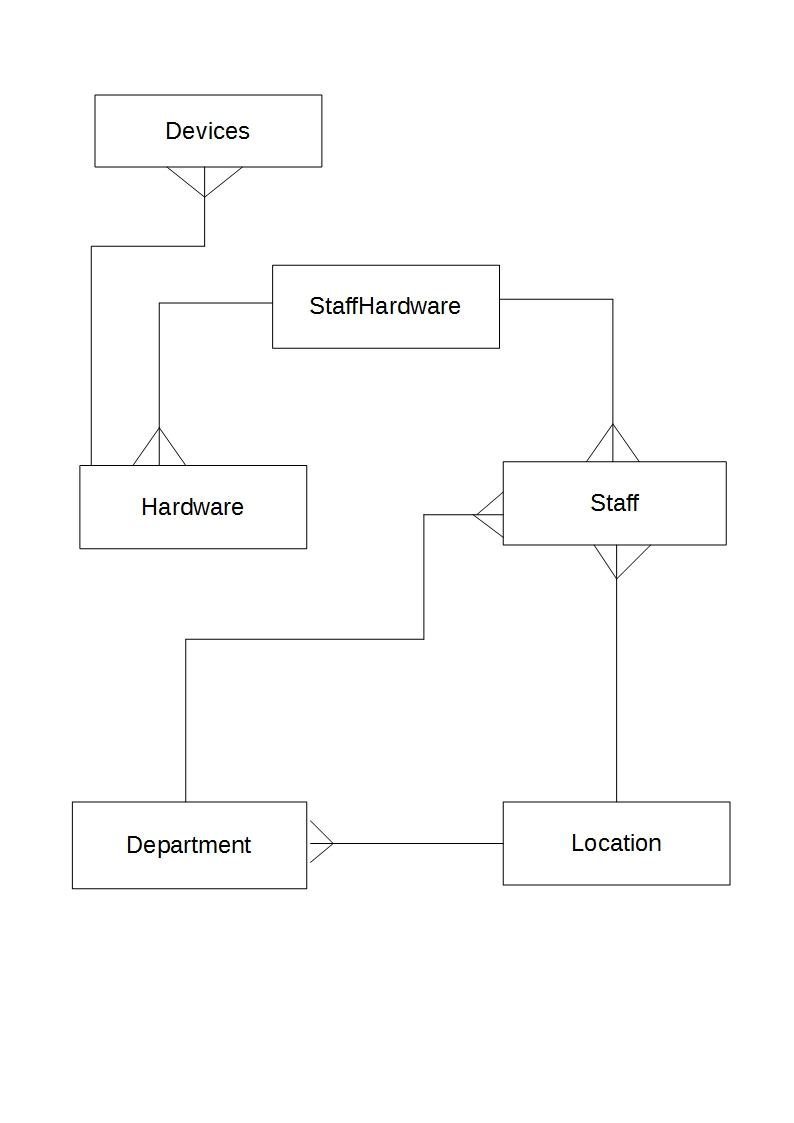
\includegraphics[width=\textwidth]{ERNormalisedDiagram.jpg}
\end{figure}


\subsubsection{Entity Descriptions}


\textbf{Staff}  (\underline{StaffID}, FirstName, LastName, JobTitle, \textit{DepartmentID},\\ \textit{ LocationID})


\

\textbf{Hardware}  (\underline{HardwareID}, \textit{DeviceID},  \textit{HardwareModelID},\\ HardwareCost, HardwareWarranty, HardwareWarrantyExpirationDate,\\ HardwareSerialNumber, 		HardwareIMEINumber, \\HardwarePhoneNumber)

\

\textbf{HardwareMake} (\underline{HardwareMakeID}, HardwareMakeName)

\

\textbf{HardwareModel} (\underline{HardwareModelID}, HardwareModelName, \textit{HardwareMakeID})

\


\textbf{DeviceType}  (\underline{DeviceID}, DeviceName)


\


\textbf{StaffHardware}  (\underline{ StaffID}, \underline{ HardwareID},PurchaseDate)


\


\textbf{Department}  (\underline{DepartmentID}, DepartmentName)


\


\textbf{Location}  (\underline{LocationID}, LocationName, LocationAddrLine1, LocationAddrLine2, LocationAddrLine3)

\

\textbf{DepartmentLocation} (\underline{LocationID}, \underline{DepartmentID})




\subsubsection{1NF to 3NF}

\begin{figure}[H]
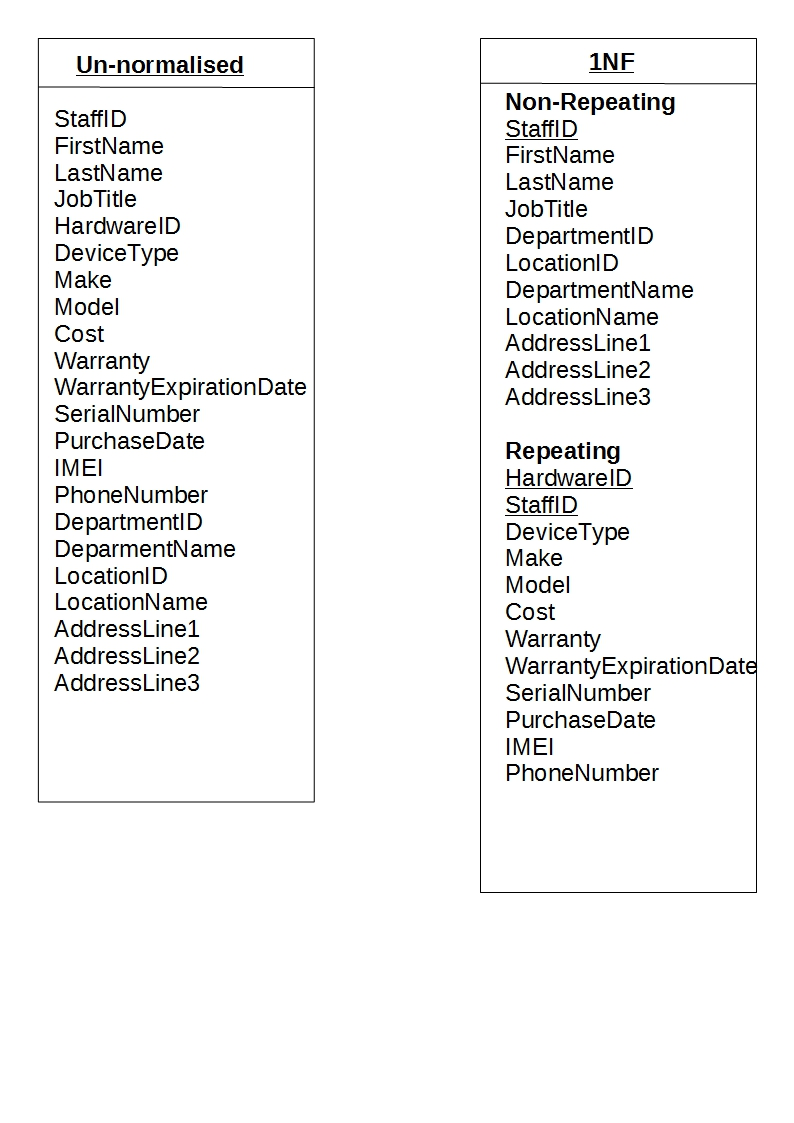
\includegraphics[width=\textwidth]{UNF&1NF.jpg}
\end{figure}

\begin{figure}[H]
\includegraphics[width=\textwidth]{2NF.jpg}
\end{figure}

\begin{figure}[H]
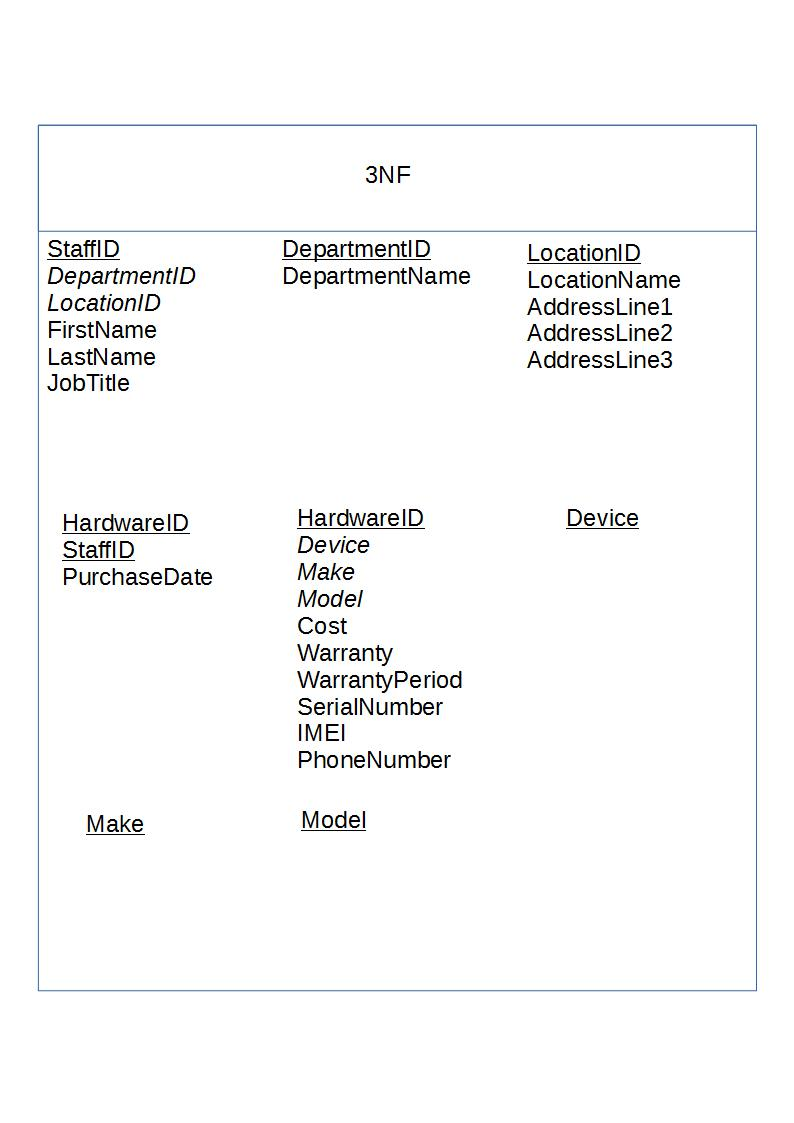
\includegraphics[width=\textwidth]{3NF.jpg}
\end{figure}

\subsection{SQL Queries}

\begin{center}
\begin{tabular}{|p{6cm}|p{5cm}|}
\hline
\textbf{SQL}      & \textbf{Description} \\ \hline
"""create table Staff(\

   StaffID INTEGER,\

   FirstName TEXT,\

   LastName TEXT,\

   JobTitle TEXT,\

   DepartmentID INTEGER,\

   LocationID INTEGER,\

   PRIMARY KEY(StaffID))\

   FOREIGN KEY(DepartmentID) \

   REFERENCES Department(DepartmentID)\

   FOREIGN KEY(LocationID) \

   REFERENCES Location(LocationID)) """                         & This SQL statement will create a new table called Staff with the attributes - StaffID, FirstName, LastName, JobTitle, DepartmentID, LocationID, The primary key is StaffID and the foreign keys are DepartmentID and LocationID                       \\ \hline

"""insert into\

Staff(FirstName,LastName, JobTitle, DepartmentID) values
(‘{'John'}’,’{'Smith'}’,’{'Data Scientist'}’,'{'5'}')
"""					 & This SQL statement will add 3 new records to the database. In this example it is entering a new staff record with attributes: FirstName, LastName, JobTitle and DepartmentID \\ \hline

"""delete from Staff\

where StaffID = ‘{3}’\

""".format(StaffID) & This statement will delete the staff member from the Staff table with the StaffID of {3} \\ \hline

"""SELECT HardwareMakeName,
From Hardware, Staff
Where HardwareID = '{0}' and StaffID = '{1}',""".format(HardwareID,StaffID) & This will fetch the HardwareMakeName the Staff with the ID of 'StaffID' has of the HardwareID of "HardwareID" \\ \hline

"""UPDATE Staff
	SET JobTitle = "Finance Manager"
	WHERE StaffID IN ("Jack",John")""" & In this example lets assume two people are being promoted at work. Both of their job titles will need changing. Here I take the job title of "Finance Manager" and apply it to both Jack and John.\\ \hline

\end{tabular}
\end{center}

\newpage

\section{Security and Integrity of the System and Data}

\subsection{Security and Integrity of Data}

This system will store somewhat personal information about staff members such as first name, last name, place of work and phone numbers. This information will fall under the data protection act so the company will have to follow the legislation. The program has an edit information function which will allow the data to be kept up to date in accordance with the data protection act. The data will also need to be encrypted to follow the legislation, my program has a login system which means the data will be stored behind a password. To make the data even more secure, ordinary staff (not managers or admin) can only see their own information as they have no need to view anyone else's. Since staff can see their own information it means they can check for incorrect personal information and using the "report incorrect information" feature they can easily notify the IT staff. This system provides a great way to deal with any incorrectly entered information. To try and avoid this validation methods will be used upon entering information. Drop down boxes will be used where possible, and boolean true or false tick boxes will be used where applicable. I will also add required fields to my database which means records will never have missing data. Lastly the login screen will have a censored password that can be changed whenever the user would like it to be.

\subsection{System Security}

The system stores a lot of data that the company will want to keep protected. It is important that the company keeps data secure and follows by the data protection act. Each member of the company has a username and password to login with which will limit the number of people being able to access the system (since only company staff can). The only way to access this data is to have a correct password and username. The database will be encrypted so the only way to access the databases is through the system. All data being entered will go through validation such as range, length checks, presence checks and drop down boxes. If the information is incorrect after the validation then it can also be edited using the edit database feature. If the information is still found to be wrong and colleague finds incorrect data about themselves they can use the "report incorrect information" (see Security and Integrity of Data above).

Because the data being stored falls under the data protection act I will need to follow the legislation principles which are as following:


\begin{center}
    \begin{tabular}{|p{5cm}|p{6cm}|}
        \hline
        \textbf{Principle} & \textbf{How To Ensure It Is Followed}\\ \hline
Personal data shall be obtained only for one or more specified and lawful purposes, and shall not be further processed in any manner incompatible with that purpose or those purposes. & The data is only held on the database for the company's use, the data will not be used anywhere else. \\ \hline
Personal data shall be adequate, relevant and not excessive in relation to the purpose or purposes for which they are processed. & Only relevant data is stored there is no need to store extra information (such as someones home address or credit card number) \\ \hline
Personal data shall be accurate and, where necessary, kept up to date. & The system includes an edit feature to allow outdated information to be changed. Validation will be in place to avoid inaccurate information \\ \hline
Personal data processed for any purpose or purposes shall not be kept for longer than is necessary for that purpose or those purposes. & If someone is to leave the company their records will be deleted as they are no longer needed \\ \hline
Appropriate technical and organisational measures shall be taken against unauthorised or unlawful processing of personal data and against accidental loss or destruction of, or damage to, personal data. & Backups will be stored with cloud storage or backup drives. Cloud storage means it cannot be accidentally destroyed \\ \hline
    \end{tabular}
\end{center}

\section{Validation}

\begin{center}
    \begin{longtable}{|p{2.5cm}|p{2cm}|p{3cm}|p{3cm}|p{3cm}|}
        \hline
        \textbf{Data Item} & \textbf{Validation} & \textbf{Presence Check?} & \textbf{Example} & \textbf{Comments} \\ \hline
StaffID                              & Range Validation \textgreater0 and \textless=350        &  Yes & 5        & This will make sure that 350 staff members can be added to the database   \\ \hline
Staff-FirstName                      & Presence Check                   & Yes        & John                  &  Ensures a name is entered                      \\ \hline
Staff-LastName                       & Presence Check               & Yes            & Smith                 &   Ensures a name is entered                     \\ \hline
StaffJobTitle			&   Length Check 			&Yes & Finance Manager		&Ensures a job title is entered and that the title is no more than 30 characters		\\ \hline
HardwareID                         &   Range Validation \textgreater0 and  \textless=300      &Yes                & 121                   & Enables up to 300 hardware devices to be added to the database \\ \hline
Hardware Cost                     &   Range Validation \textgreater0 and \textless=2000            &Yes                        & £500                  &  The cost of a hardware item will not be more than 2000                     \\ \hline
Hardware Warranty                    & Presence Check            &Yes               & True                  & Ensures a True/False statement is entered                      \\ \hline
Hardware Warranty ExpirationDate           & Format                      &No             & 11/03/2017               &   Ensures the date is entered in the correct format. This will automatically be entered when the user clicks the calender date                    \\ \hline
Hardware SerialNumber              & Length                 &Yes                  & 12307321              &      Ensures no more than 40 characters are entered                 \\ \hline
Hardware PurchaseDate               & Format                 &No                  & 11/03/2015              & Ensures the date is entered in the correct format. This will automatically be entered when the user clicks the calender date                       \\ \hline
Hardware-IMEI               & Length              &Yes                     & EH37000781               & Ensures a length of up to 30 characters                      \\ \hline
Hardware PhoneNumber                  & Length            &Yes                      & 07927551125              &   Ensures only 11 chracters are entered                      \\ \hline
DeviceID                     & Range Validation \textgreater0 and \textless=100            &Yes                       & 24                 & This allows 100 different devices to be added to the database                    \\ \hline
DeviceName                         & Length                       &Yes            & Phone, Laptop, Tablet                &  Ensures a length of a device is not more than 15 characters                     \\ \hline
Hardware MakeID                    & Range Validation \textgreater0 and \textless=200      &Yes                             & 24                 & 200 different models can be entered into the database                       \\ \hline
Hardware Make                        & Length               &Yes                    & iPhone                & Ensures the length of a make is not more than 15 characters                      \\ \hline
Hardware ModelID		& Range Validation \textgreater0 and \textless=300                      &Yes             & 24                 & Allows for 300 models to be entered into the database                        \\ \hline
Hardware Model                      & Length            &Yes                       & 5S                    & Ensures no more than 15 characters will be entered                       \\ \hline
DepartmentID 	&Range Validation \textgreater0 and \textless=75	&Yes	& 24		& Allows for 75 departments to be added to the database	\\ \hline
Department Name	& Length	&Yes	& Financing		& Allows for 25 characters to be entered for the department	\\ \hline
LocationID 		&Range Validation \textgreater0 and \textless=20	&Yes	& 	24	& 20 work locations can be entered		\\ \hline
Location Name	& Length	&Yes	&	Orwell	 & No more than 25 characters can be entered for the location  \\ \hline
Location AddrLine1 & Length	&Yes	&	50 Fisher's Ln	 & Up to 50 characters may be entered for address line 1  \\ \hline
Location AddrLine2 & Length	&No	&	Orwell	 & Up to 15 characters may be entered for address line 2 \\ \hline
Location AddrLine3  & Length	&No	&	Royston 	 &Up to 15 characters may be entered for address line 3  \\ \hline
    \end{longtable}
\end{center}

\section{Testing}

\begin{landscape}
\subsection{Outline Plan}

\begin{center}
    \begin{tabular}{|p{2cm}|p{5cm}|p{5cm}|p{4cm}|}
        \hline
        \textbf{Test Series} & \textbf{Purpose of Test Series} & \textbf{Testing Strategy} & \textbf{Strategy Rationale}\\ \hline
1 & Test flow of control between the user interfaces & Top-down testing & A outline of the GUI will be developed and once working more modules will be added \\ \hline
       2 & To test validation of input data is performed correctly & Bottom-up testing & Components will be tested as they become available \\ \hline
3 & To test if the data is stored in its correct location & Black box testing & An output that the program produces will be examined for correctness and then the next output can be examined.\\ \hline
4 & To check information can be read from the database and read through the system & Bottom-up testing &  Components will be tested as they become available\\ \hline
5 & Check that the system cannot have unauthorised access & Unit testing & To test individual software components \\ \hline
6 & To check the finished system will fulfil the specifications &  Acceptance Testing & Performed by the client to check the system meets their requirements\\ \hline

    \end{tabular}
\end{center}

\subsection{Detailed Plan}

\begin{center}
    \begin{longtable}{|p{1.5cm}|p{2.5cm}|p{2.5cm}|p{2cm}|p{2cm}|p{2cm}|p{2cm}|p{2cm}|}
        \hline
        \textbf{Test Series} & \textbf{Purpose of Test} & \textbf{Test Description} & \textbf{Test Data} & \textbf{Test Data Type (Normal/ Erroneous/ Boundary)} & \textbf{Expected Result} & \textbf{Actual Result} & \textbf{Evidence}\\ \hline
1.01 & Test the manager login button on the select login page to ensure it works correctly  & This takes the user to the appropriate login screen & Click the Manager Login button & Normal & The manager login screen should be displayed && \\ \hline
1.02 & Test the staff login button on the select login page to ensure it works corrently & This takes the user to the appropriate login screen & Click the Staff Login button & Normal & The staff login screen should be displayed && \\ \hline
1.03 & Test the staff admin button on the select login page to ensure it works corrently & This takes the user to the appropriate login screen & Click the Admin Login button & Normal & The admin login screen should be displayed && \\ \hline
1.04 & Test the log in button on the manager login screen  & This takes the user to the appropriate main menu & Click the Log In button on the manager login screen & Normal & The manager main menu screen displayed && \\ \hline
1.05 & Test the log in button on the staff login screen  & This takes the user to the appropriate main menu & Click the Log In button on the staff login screen & Normal & The staff main menu screen displayed && \\ \hline
1.05 & Test the log in button on the admin login screen  & This takes the user to the appropriate main menu & Click the Log In button on the admin login screen & Normal & The admin main menu screen displayed && \\ \hline
1.06 & Test the forgot password button on the login screens & Takes the user to password recovery & Click the forgot password button & Normal & The password recovery form will be displayed && \\ \hline
1.07 & Test the submit button on the password recovery form & After the user enters form details they will click this to send it to IT staff & Click the submit button & Normal & An email will be sent to the IT staff (or the email specified) && \\ \hline
1.08 & Test the view department  button on the manager homepage & Will take the user to view their department information & Click the view department button & Normal & The layout will be switched to the staff database showing only people in their department && \\ \hline
1.09 & Test the view my information button on the manager homepage & Will take the user to view their own information & Click the view own information button& Normal  & The layout will be switched to the staff database showing only their own information && \\ \hline
1.10 & Test the cancel button on the change password screen & No changes will be saved & Click the cancel button & Normal & The window will close && \\ \hline
1.11 & Test the change button on the change password screen & Changes will be saved & Click the change button & Normal & The window will close and changes will be saved&& \\ \hline
1.12 & Test the cancel button on the report bug screen & Changes will not be saved & Click the cancel button & Normal & The window will close&& \\ \hline
1.13 & Test the submit button on the report bug screen & Changes will be saved and the form will be sent to IT staff & Click the submit button& Normal  & The window will close and an email will be sent to IT staff with all details (or the email specified) && \\ \hline
1.14 & Test the cancel button on the report errors screen & Changes will not be saved & Click the cancel button & Normal & The window will close&& \\ \hline
1.15 & Test the submit button on the report errors screen & Changes will be saved and the form will be sent to IT staff & Click the submit button& Normal  & The window will close and an email will be sent to IT staff with all details (or the email specified) && \\ \hline
1.16 & Test the open database button on the admin home screen & The open database screen should open & Click the open database button& Normal  & The window should switch layouts to the open database screen && \\ \hline
1.17 & Test the search for staff button on the admin home screen & The search staff screen should open & Click the search staff button& Normal  & The window should switch layouts to the search staff screen && \\ \hline
1.18 & Test the close button on the staff information (search staff screen) & The window will close  & Click the close button& Normal  & The window should close and return to the search screen && \\ \hline
1.19 & Test the edit database button on the open database screen & To test whether the edit buttons will shown up  & Click the edit database button& Normal  & Buttons to edit the data should show up && \\ \hline
1.20 & Test the edit button on the edit database screen & To test whether the edit buttons will open up a edit screen  & Click a edit button& Normal  & A new screen will appear allowing the user to enter information && \\ \hline
1.21 & Test the save changes button on the edit database input screen & To test whether the save changes button will save the changes made  & Click a save changes button& Normal  & The screen will close but changes will have applied && \\ \hline
1.22 & Test the add data button on the open database screen & To test whether screen to input data will show up  & Click the add data button& Normal  & The window to add data to the database will show up && \\ \hline
1.23 & Test the add data button on the data input screen & To test whether data will be added to the database  & Click the add data button& Normal  & The window will close and the data entered will have been added to the database && \\ \hline
1.24 & Test the remove data button on the open database screen & To test whether delete buttons will show up next to the records in the database  & Click the remove data button& Normal  & The delete buttons will show up next to each record && \\ \hline
1.25 & Test the delete buttons on the delete data screen & To test whether delete buttons will display a message  & Click a delete data button & Normal  & A warning sign should show up to confirm the user would like to remove the selected data && \\ \hline
1.26 & Test the no button on the delete data warning window & To test whether the no button will keep the data from being deleted  & Click the no data button & Normal  & The warning window will close and return to the previous screen. && \\ \hline
1.27 & Test the yes button on the delete data warning window & To test whether the yes button will delete the data selected  & Click the yes data button & Normal  & The warning window will close and return to the previous screen with the specified data deleted . && \\ \hline

1.28 & Test the Help menu (on Staff and Manager GUI) & To test whether a dropdown list of buttons will show up  & Click the help menu & Normal  & The menu should function correctly and display the "report bug" and "report incorrect information" buttons . && \\ \hline
1.29 & Test the Help menu buttons (on Staff and Manager GUI) & To test whether the buttons will work on the help menu  & Click the report bug and report incorrect information buttons & Normal  & The "report bug" should take the user to the report bug screen and "report incorrect information" should take the user to the report incorrect information screen . && \\ \hline

1.30 & Test the Account menu & To test whether a dropdown list of buttons will show up  & Click the account menu & Normal  & The menu should function correctly and display the "log out" and "change password" buttons . && \\ \hline
1.31 & Test the Account menu buttons & To test whether the buttons will work on the account menu  & Click the log out and change password buttons & Normal  & The "log out" should take the user back to the intitial login screen and "change password" should take the user to the change password screen . && \\ \hline

1.32 & Test the View menu (on Manager GUI)  & To test whether a dropdown list of buttons will show up  & Click the view menu & Normal  & The menu should function correctly and display the "department database" and "your information" buttons . && \\ \hline
1.33 & Test the View menu buttons (on Manager GUI) & To test whether the buttons will work on the view menu  & Click the department database and your information buttons & Normal  & The "department database" should take the user to the department database screen "your information" should take the staff database showing only your information . && \\ \hline

1.34 & Test the Database menu (on Admin GUI)  & To test whether a dropdown list of buttons will show up  & Click the Database menu & Normal  & The menu should function correctly and display "Staff", "Hardware", "Location" and "Department"  which all have secondary buttons to view, edit, add and remove data&& \\ \hline
1.35 & Test the Database menu buttons (on Admin GUI) & To test whether the buttons will work on the database menu coming off of  "Staff", "Hardware", "Location" and "Department"  & Click each button & Normal  & Each button will take the user to the specified database and either the normal view screen, edit screen, add data screen or remove data screen && \\ \hline

1.36 & Test the arrow buttons on the seach staff screen & To test whether the buttons next to each record will open a new window to view more information  & Click each button & Normal  & Any button should open up a screen to display more information about a staff member && \\ \hline

1.37 & Test the return to database view button on the open database screen & After Edit, Add or Remove is clicked the user may click this button to return to the viewing mode & Click return to database view button & Normal  & The layout will change to the normal view. && \\ \hline

1.38 & Test the back button on the admin interfaces & These buttons will take the user back to the home page & Click the return button & Normal  & The layout will change to the admin home page. && \\ \hline

2.1 & Test the dropdown boxes for department selection & To test whether the drop down boxes will function corrently on the open database and the search staff page. The options must actually open that database  & Click each button on the dropdown box & Normal  & Each button should open the database wanted && \\ \hline
2.2 & Test the dropdown boxes for data input windows (e.g. location and department) & To test whether the drop down boxes will function corrently when inputting data. The options must actually fill in the boxes once clicked  & Click each button on the dropdown box & Normal  & Each button should fill the box with the selection chosen && \\ \hline

2.3 & Test the calender works for date inputs & To test whether the calender will open when the icon is clicked. Once a date is selected it should automatically fill the box. & Click a date on the calender & Normal  & The date should be entered once a date on the calender is clicked in the following format DD/MM/YYYY && \\ \hline
2.4 & Verify that the username field has between 3 - 12 characters in it & The field cannot be blank, it has to have more than 3 characters but no more than 12. & Nothing \ 30597 \ JSmith21 \ JordanSumerfield &Erroneous \ Normal \ Normal \ Erroneous & Error         \par Valid              \par Valid                 \par Error && \\ \hline
2.5 & Verify that the password field has between 6 - 20 characters in it & The field cannot be blank, it has to have more than 6 characters but no more than 20. & Nothing \par\ password \par pA33WoRD \par cat  &Erroneous \par Normal \par Normal \par Erroneous & Error         \par Valid              \par Valid                 \par Error && \\ \hline
2.6 & Verify Email, Forename, Surname is entered in recover password fields & The fields cannot be blank and must have a '@' symbol in the email address. & John, Smith, J.com \par John, Smith, J@gmail.com \par JJ, D, JJD@hotmail.com \par & Erroneous \par Valid \par Valid \\ \hline
2.7 & Verify Email, Forename, Surname, Job Title, Date and Details of bug are entered in the report bug page & All fields must have some data in them before the submit  button is clicked & All fields filled out apart from Details of bug \par All details filled out & Erroneous \par Normal & Error \par Valid && \\ \hline
2.8 & Verify Email, Forename, Surname and description are entered in the report errors page & All fields must have some data in them before the submit  button is clicked & All fields filled out apart from forename \par All details filled out & Erroneous \par Normal & Error \par Valid && \\ \hline

3.1 & Verify the Staff details are entered correctly into the Staff database & All information should be added to the required fields  & Staff information & Normal& Data is added to Staff table && \\ \hline
3.2 & Verify the Hardware details are entered correctly into the Hardware database & All information should be added to the required fields  &Hardware information & Normal& Data is added to Hardware table && \\ \hline
3.3 & Verify the Location details are entered correctly into the Location database & All information should be added to the required fields  &Location information & Normal& Data is added to Location table && \\ \hline
3.4 & Verify the Department details are entered correctly into the Department database & All information should be added to the required fields  &Department information & Normal& Data is added to Department table && \\ \hline
3.5 & Verify the DeviceType details are entered correctly into the DeviceType database & All information should be added to the required fields  &DeviceType information & Normal& Data is added to DeviceType table && \\ \hline
3.6 & Verify the HardwareMake details are entered correctly into the HardwareMake database & All information should be added to the required fields  &HardwareMake information & Normal& Data is added to HardwareMake table && \\ \hline
3.7 & Verify the HardwareModel details are entered correctly into the HardwareModel database & All information should be added to the required fields  &HardwareModel information & Normal& Data is added to HardwareModel table && \\ \hline
3.8 & Verify the Staff's Hardware details with purchase date are entered correctly into the StaffHardware database & All information should be added to the required fields  &StaffHardware information & Normal& Data is added to StaffHardware table && \\ \hline
3.9 & Verify the DepartmentLocation details with purchase date are entered correctly into the DepartmentLocation database & All information should be added to the required fields  &DepartmentLocation information & Normal& Data is added to DepartmentLocation table && \\ \hline

4 & Verify each table can be read by clicking the dropdown box and selecting the database wanted & Each table should be able to be clicked and be viewed in a table format&Data from the following tables: \par Staff \par Hardware \par Location \par Department \par DeviceType \par HardwareMake \par HardwareModel \par StaffHardware \par DepartmentLocation & Normal& The table will be shown and will match information in the database && \\ \hline

5.1 & Check that staff members cannot log in to managers or admins interfaces & Staff should not be able to use their login to access the admin interface or the manager interface, only their own. & Staff login details & Erroneous & The system will say incorrect login details && \\ \hline
5.2 & Check that managers cannot log in to staff or admins interfaces & managers should not be able to use their login to access the admin interface or the staff interface, only their own. & managers login details & Erroneous & The system will say incorrect login details && \\ \hline
5.2 & Check that admins cannot log in to staff or managers interfaces & admins should not be able to use their login to access the manager interface or the staff interface, only their own. & admins login details & Erroneous & The system will say incorrect login details && \\ \hline

6 & Verify the program fulfils all the specifications & Run through the program testing every aspect with correct and incorrect data to insure all the objectives are met & Normal &The program should fulfil all specifications and objectives && \\ \hline

%##################### GOT TO FIGURE 2.9 on buttons
    \end{longtable}
\end{center}
\end{landscape}
